%% =====================================================================
%%  BCSE497J Project Report -- OrchardVision
%%  Built from the VIT Chennai BCSE497J report template.
%%
%%  MARKER CONVENTION
%%    \add{...}  = content beyond the project documentation
%%    \ph{...}   = placeholder to fill before submission
%%    \pp{...}   = value to fill before submission (prints as <<VALUE>>)
%%    \hr        = table-row marker (put first in the row)
%%    No colour is applied to any of these; the macros are pass-through.
%% =====================================================================
\documentclass[12pt,a4paper]{report}

% ---------- page geometry (template: L 3.81cm, R/T/B 2.54cm, A4) ----------
\usepackage[left=3.81cm,right=2.54cm,top=2.54cm,bottom=2.54cm]{geometry}

% ---------- fonts: Times, 12pt ----------
\usepackage[T1]{fontenc}
\usepackage[utf8]{inputenc}
\usepackage{mathptmx}
\usepackage{microtype}

% ---------- packages ----------
\usepackage{setspace}
\usepackage{graphicx}
\usepackage{xcolor}
\usepackage{colortbl}
\usepackage{booktabs}
\usepackage{longtable}
\usepackage{array}
\usepackage{tabularx}
\usepackage{enumitem}
\usepackage{listings}
\usepackage{caption}
\usepackage{fancyhdr}
\usepackage{titlesec}
\usepackage{tocloft}
\usepackage{amsmath}
\usepackage{float}
\usepackage[obeyspaces,spaces]{url}
\usepackage{tikz}
\usetikzlibrary{arrows.meta,positioning,shapes.geometric,fit,calc}
\usepackage[hidelinks]{hyperref}
\urlstyle{tt}
\def\UrlBreaks{\do\/\do\_\do\-\do\.\do\{\do\}}

% ---------- marker macros (no highlighting; kept so chapters compile unchanged) ----------
% \emphon{} ... \emphoff{}  : italic span inside \add{...}
\newcommand{\emphon}{\itshape}
\newcommand{\emphoff}{\upshape}
% \add{...}  : text contributed beyond the project documentation
\newcommand{\add}[1]{#1}
% \ph{...}   : placeholder to fill before submission
\newcommand{\ph}[1]{#1}
% \hr        : table-row marker (put first in the row)
\newcommand{\hr}{}
\newcommand{\pp}[1]{\textless\kern0pt\textless{}#1\textgreater\kern0pt\textgreater{}}
% code / path in text
\newcommand{\code}[1]{\path{#1}}
\def\phcol{white}

% image placeholder: label, short caption, long caption, description, height
\newcommand{\figph}[5]{%
  \begin{figure}[htbp]
    \centering
    \fcolorbox{black}{\phcol}{\parbox[c][#5][c]{0.92\linewidth}{\centering\small
      \textbf{[IMAGE PLACEHOLDER]}\\[3pt]#4}}
    \caption[#2]{\add{#3}}\label{#1}
  \end{figure}}

% ---------- spacing ----------
\onehalfspacing
\setlength{\parindent}{0pt}
\setlength{\parskip}{6pt plus 1pt}
\tolerance=2500
\emergencystretch=3em
\widowpenalty=10000
\clubpenalty=10000
\setlist{itemsep=2pt,topsep=4pt,parsep=0pt}

% ---------- headings (template: chapter 16 bold; section 14 CAPS; subsection 12 CAPS) ----------
\titleformat{\chapter}[display]
  {\centering\bfseries\fontsize{16}{20}\selectfont}
  {\MakeUppercase{\chaptername}\ \thechapter}{8pt}{\MakeUppercase}
\titleformat{name=\chapter,numberless}[display]
  {\centering\bfseries\fontsize{16}{20}\selectfont}{}{0pt}{\MakeUppercase}
\titlespacing*{\chapter}{0pt}{0pt}{18pt}
\titleformat{\section}
  {\bfseries\fontsize{14}{17}\selectfont}{\thesection}{0.8em}{\MakeUppercase}
\titleformat{\subsection}
  {\bfseries\fontsize{12}{15}\selectfont}{\thesubsection}{0.8em}{\MakeUppercase}
\titleformat{\subsubsection}
  {\bfseries\fontsize{12}{15}\selectfont}{\thesubsubsection}{0.8em}{}
\titlespacing*{\section}{0pt}{14pt plus 2pt}{6pt}
\titlespacing*{\subsection}{0pt}{10pt plus 2pt}{4pt}
\titlespacing*{\subsubsection}{0pt}{8pt plus 2pt}{3pt}

% ---------- page numbers: bottom centre ----------
\pagestyle{fancy}
\fancyhf{}
\fancyfoot[C]{\thepage}
\renewcommand{\headrulewidth}{0pt}
\fancypagestyle{plain}{\fancyhf{}\fancyfoot[C]{\thepage}\renewcommand{\headrulewidth}{0pt}}

% ---------- captions (>= 10pt) ----------
\captionsetup{font=small,labelfont=bf,skip=6pt}
\renewcommand{\arraystretch}{1.15}

% ---------- code listings ----------
\lstdefinestyle{plain}{basicstyle=\ttfamily\footnotesize,breaklines=true,frame=single,
  columns=fullflexible,keepspaces=true,xleftmargin=4pt,xrightmargin=4pt,
  showstringspaces=false,aboveskip=6pt,belowskip=6pt}
\lstdefinestyle{added}{style=plain,backgroundcolor=\color{\phcol}}

% ---------- headings for front matter ----------
\newcommand{\fronthead}[1]{%
  \begin{center}\underline{\textbf{\fontsize{14}{17}\selectfont #1}}\end{center}\vspace{6pt}}

% ---------- candidate / guide details (EDIT HERE) ----------
\newcommand{\projtitle}{Video-Based Fruit Counting with Tracking to Eliminate Double-Counting}
\newcommand{\candname}{DERRICK SAMUEL R.}
\newcommand{\candreg}{23BCE1040}
\newcommand{\candtwoname}{PRANNAVAKHANTH}
\newcommand{\candtworeg}{23BCE1869}
\newcommand{\candthreename}{PRIYANKA KALIRAJ}
\newcommand{\candthreereg}{23BCE5131}
\newcommand{\candall}{\candname\ (\candreg),\ \candtwoname\ (\candtworeg), and \candthreename\ (\candthreereg)}
\newcommand{\guidename}{Dr. Manas Ranjan Prusty}
\newcommand{\guidedesig}{Associate Professor Grade 2}
\newcommand{\hodname}{Dr. Prassanna Jayachandran}
\newcommand{\specname}{Core}
\newcommand{\submitdate}{November, 2026}

\begin{document}

%% ====================== 1. COVER PAGE ======================
\pagestyle{empty}
\begin{titlepage}
\centering\singlespacing
{\itshape\fontsize{12}{15}\selectfont A project report on\par}
\vspace{16pt}
{\bfseries\fontsize{20}{26}\selectfont \projtitle\par}
\vspace{16pt}
{\itshape\fontsize{14}{18}\selectfont Submitted in partial fulfillment for the award of the degree of\par}
\vspace{12pt}
{\bfseries\fontsize{22}{27}\selectfont Bachelor of Technology in\\ Computer Science and Engineering Core\\ \par}
\vspace{14pt}
{\itshape\fontsize{14}{18}\selectfont by\par}
\vspace{10pt}
{\bfseries\fontsize{16}{20}\selectfont \candname\ (\candreg)\par}
\vspace{4pt}
{\bfseries\fontsize{16}{20}\selectfont \candtwoname\ (\candtworeg)\par}
\vspace{4pt}
{\bfseries\fontsize{16}{20}\selectfont \candthreename\ (\candthreereg)\par}
\vfill

\includegraphics[width=3.26in]{vit_logo.png}\par
\vspace{14pt}
{\bfseries\fontsize{16}{20}\selectfont SCHOOL OF COMPUTER SCIENCE AND ENGINEERING\par}
\vspace{6pt}
{\fontsize{12}{15}\selectfont \submitdate\par}
\end{titlepage}

%% ====================== 2. TITLE PAGE ======================
\begin{titlepage}
\centering\singlespacing
{\itshape\fontsize{12}{15}\selectfont A project report on\par}
\vspace{16pt}
{\bfseries\fontsize{20}{26}\selectfont \projtitle\par}
\vspace{16pt}
{\itshape\fontsize{14}{18}\selectfont Submitted in partial fulfillment for the award of the degree of\par}
\vspace{12pt}
{\bfseries\fontsize{22}{27}\selectfont Bachelor of Technology in\\ Computer Science and Engineering Core\\ \par}
\vspace{14pt}
{\itshape\fontsize{14}{18}\selectfont by\par}
\vspace{10pt}
{\bfseries\fontsize{16}{20}\selectfont \candname\ (\candreg)\par}
\vspace{4pt}
{\bfseries\fontsize{16}{20}\selectfont \candtwoname\ (\candtworeg)\par}
\vspace{4pt}
{\bfseries\fontsize{16}{20}\selectfont \candthreename\ (\candthreereg)\par}
\vfill

\includegraphics[width=3.26in]{vit_logo.png}\par
\vspace{14pt}
{\bfseries\fontsize{16}{20}\selectfont SCHOOL OF COMPUTER SCIENCE AND ENGINEERING\par}
\vspace{6pt}
{\fontsize{12}{15}\selectfont \submitdate\par}
\end{titlepage}

%% ====================== 3. DECLARATION ======================
\newpage
\begin{center}
\includegraphics[width=3.26in]{vit_logo.png}\end{center}
\fronthead{DECLARATION}
I hereby declare that the thesis entitled ``\projtitle'' submitted by \candthreename\ (\candthreereg), for the award of the degree of Bachelor of Technology in Computer Science and Engineering, Vellore Institute of Technology, Chennai is a record of bonafide work carried out by me under the supervision of \guidename.

I further declare that the work reported in this thesis has not been submitted and will not be submitted, either in part or in full, for the award of any other degree or diploma in this institute or any other institute or university.

\vspace{30pt}
\noindent Place: Chennai\hfill\textbf{Signature of the Candidate}\\[6pt]
Date:

%% ====================== 4. CERTIFICATE ======================
\newpage
\begin{center}
\includegraphics[width=3.26in]{vit_logo.png}\\[4pt]
{\bfseries School of Computer Science and Engineering}\end{center}
\fronthead{CERTIFICATE}
This is to certify that the report entitled \textbf{``\projtitle''} is prepared and submitted by \candthreename\ (\candthreereg)\ to Vellore Institute of Technology, Chennai, in partial fulfillment of the requirement for the award of the degree of \textbf{Bachelor of Technology in Computer Science and Engineering Core} is a bonafide record carried out under my guidance. The project fulfills the requirements as per the regulations of this University and in my opinion meets the necessary standards for submission. The contents of this report have not been submitted and will not be submitted either in part or in full, for the award of any other degree or diploma and the same is certified.

\vspace{18pt}
\noindent Signature of the Guide:\\[6pt]
Name: \ \guidename\\[6pt]
Date:

\vspace{22pt}
\noindent\begin{tabular}{@{}p{0.48\textwidth}p{0.48\textwidth}@{}}
Signature of the Examiner & Signature of the Examiner\\[8pt]
Name: Dr. Renta Chintala Bhargavi & Name: Dr. Ranjith R\\[8pt]
Date: & Date:
\end{tabular}

\vspace{20pt}
\noindent\begin{tabular}{@{}p{0.48\textwidth}p{0.48\textwidth}@{}}
& Approved by the Head of Department, \\[-2pt]
& \textbf{B.Tech.\ Computer Science and} \\[-2pt]
& \textbf{Engineering \specname} \\[14pt]
& Signature\hspace{4cm} \\[6pt]
& Name: \textbf{\hodname} \\[6pt]
& Date:
\end{tabular}

%% (Certificate by External Guide -- only for PAT-discontinued students -- omitted;
%%  insert here if applicable.)

%% ====================== FRONT MATTER (roman numerals) ======================
\clearpage
\pagestyle{fancy}
\pagenumbering{roman}
\setcounter{page}{1}

%% ====================== ABSTRACT ======================
\fronthead{ABSTRACT}
OrchardVision is a computer vision system for long-term fruit tracking and counting in mango orchards. It implements identity learning, tracking pipelines, and a full-stack web interface for experiment management and video processing.

Estimating the number of fruit on a tree or across a block is central to yield forecasting, harvest logistics and crop-load management, yet it is still largely done by manual sampling. Counting from orchard video is attractive but difficult: fruit are small, visually similar, frequently hidden by leaves and branches, and the same fruit re-enters the camera view many times as the camera moves along a row or revisits it on later days. A detector-only counter therefore double-counts, and a frame-to-frame tracker alone loses identities whenever a fruit is occluded.

The system developed in this project is built around a processing pipeline that orchestrates frame extraction, object detection, tracking (mock, ByteTrack or TAPNext backends), re-identification embeddings, identity consolidation and analytics. Each fruit is represented by an identity prototype (an embedding vector with quality and observation statistics), so that a fruit that disappears and later reappears can be re-associated with the same identity. Camera motion is estimated and compensated, and tracking quality is reported using IDF1, HOTA and identity-switch metrics. The backend is a FastAPI service with a SQLAlchemy~2.0 data layer (SQLite for development, PostgreSQL for production) and S3-compatible object storage; the frontend is a React and TypeScript application sharing typed contracts with the API. An experiment harness lets users run and compare tracker configurations and export results as JSON or CSV.

The report presents the motivation, related work, requirements, architecture, data model, pipeline design, API design, deployment and testing approach of OrchardVision, followed by an evaluation plan with placeholders for the quantitative results and a discussion of limitations and future work.

\vspace{6pt}
\noindent\textbf{Keywords:} \add{fruit counting; multi-object tracking; re-identification; identity learning; precision agriculture; mango orchard; FastAPI; React.}

%% ====================== ACKNOWLEDGEMENT ======================
\clearpage
\fronthead{ACKNOWLEDGEMENT}
It is my pleasure to express with deep sense of gratitude to \guidename, \guidedesig, School of Computer Science and Engineering, Vellore Institute of Technology, Chennai, for his constant guidance, continual encouragement, understanding; more than all, he taught me patience in my endeavor. My association with him is not confined to academics only, but it is a great opportunity on my part of work with an intellectual and expert in the field of \add{computer vision and machine learning}.

It is with gratitude that I would like to extend my thanks to the visionary leader Dr. G. Viswanathan our Honorable Chancellor, Mr. Sankar Viswanathan, Dr. Sekar Viswanathan, Dr. G V Selvam Vice Presidents, Dr. Sandhya Pentareddy, Executive Director, Ms. Kadhambari S. Viswanathan, Assistant Vice-President, Dr. V. S. Kanchana Bhaaskaran Vice-Chancellor, Dr. T. Thyagarajan Pro-Vice Chancellor, VIT Chennai and Dr. P. K. Manoharan, Additional Registrar for providing an exceptional working environment and inspiring all of us during the tenure of the course.

Special mention to Dr. Viswanathan V, Dean, Dr. Nithyanandam P, Associate Dean, Dr. Suganya G, Associate Dean, Dr. Sweetlin Hemalatha C, Associate Dean, School of Computer Science and Engineering, Vellore Institute of Technology, Chennai for spending their valuable time and efforts in sharing their knowledge and for helping us in every aspect.

In jubilant state, I express ingeniously my whole-hearted thanks to \textbf{\hodname}, Head of the Department, B.Tech.\ \textbf{Computer Science and Engineering (\specname)} and the Project Coordinators for their valuable support and encouragement to take up and complete the thesis.

My sincere thanks to all the faculties and staffs at Vellore Institute of Technology, Chennai who helped me acquire the requisite knowledge. I would like to thank my parents for their support. It is indeed a pleasure to thank my friends who encouraged me to take up and complete this task.

\vspace{18pt}
\noindent Place: Chennai\hfill\textbf{\candthreename}\\
Date:

%% ====================== CONTENTS, LISTS ======================
\clearpage
\renewcommand{\contentsname}{CONTENTS}
\renewcommand{\listtablename}{LIST OF TABLES}
\renewcommand{\listfigurename}{LIST OF FIGURES}
\renewcommand{\cftchapfont}{\bfseries}
\renewcommand{\cftchappagefont}{\bfseries}
\renewcommand{\cftchappresnum}{\MakeUppercase{\chaptername}\ }
\setlength{\cftchapnumwidth}{6.6em}
\setlength{\cftsecindent}{1.5em}
\setlength{\cftsecnumwidth}{2.5em}
\setlength{\cftsubsecindent}{4em}
\setlength{\cftsubsecnumwidth}{3.2em}
\setlength{\cftfignumwidth}{2.6em}
\setlength{\cfttabnumwidth}{2.6em}
{\singlespacing
\addcontentsline{toc}{chapter}{CONTENTS}
\tableofcontents
\clearpage
\listoffigures
\addcontentsline{toc}{chapter}{LIST OF FIGURES}
\clearpage
\listoftables
\addcontentsline{toc}{chapter}{LIST OF TABLES}
\clearpage
}

\chapter*{List of Acronyms}
\addcontentsline{toc}{chapter}{LIST OF ACRONYMS}
{\singlespacing
\begin{longtable}{@{}p{3.2cm}p{10.9cm}@{}}
\hr \textbf{API} & Application Programming Interface\\
\hr \textbf{CORS} & Cross-Origin Resource Sharing\\
\hr \textbf{CSV} & Comma-Separated Values\\
\hr \textbf{FPS} & Frames Per Second\\
\hr \textbf{HOTA} & Higher Order Tracking Accuracy\\
\hr \textbf{IDF1} & Identification F1 score\\
\hr \textbf{IDSW} & Identity Switches (ID switches)\\
\hr \textbf{JSON} & JavaScript Object Notation\\
\hr \textbf{MOT} & Multi-Object Tracking\\
\hr \textbf{ORM} & Object-Relational Mapping\\
\hr \textbf{PCA} & Principal Component Analysis\\
\hr \textbf{ReID} & Re-Identification\\
\hr \textbf{REST} & Representational State Transfer\\
\hr \textbf{SQL} & Structured Query Language\\
\hr \textbf{TAP} & Tracking Any Point\\
\hr \textbf{t-SNE} & t-distributed Stochastic Neighbour Embedding\\
\hr \textbf{UI} & User Interface\\
\hr \textbf{UUID} & Universally Unique Identifier\\
\end{longtable}}

\chapter*{List of Symbols and Nomenclature}
\addcontentsline{toc}{chapter}{LIST OF SYMBOLS AND NOMENCLATURE}
{\singlespacing
\begin{longtable}{@{}p{3.2cm}p{10.9cm}@{}}
\hr $\mathbf{e}_t$ & \add{ReID embedding extracted from a detection at frame $t$}\\
\hr $\mathbf{p}_k$ & \add{Prototype (memory) embedding of identity $k$}\\
\hr $\alpha$ & \add{Memory update rate used when a prototype is refreshed}\\
\hr $\tau_{\mathrm{reid}}$ & \add{ReID similarity threshold for accepting a re-association}\\
\hr $\tau_{\mathrm{conf}}$ & \add{Detection confidence threshold}\\
\hr $\tau_{\mathrm{match}}$ & \add{Tracker match threshold}\\
\hr $\mathrm{IDTP},\mathrm{IDFP},\mathrm{IDFN}$ & \add{Identity-level true positives, false positives and false negatives}\\
\hr $\mathrm{HOTA}_\beta$ & \add{HOTA score at localisation threshold $\beta$}\\
\hr $\mathrm{DetA},\mathrm{AssA}$ & \add{Detection accuracy and association accuracy components of HOTA}\\
\end{longtable}}


%% ====================== MAIN MATTER (arabic) ======================
\clearpage
\pagenumbering{arabic}
\setcounter{page}{1}

\chapter{Introduction}

\section{Introduction}

OrchardVision is a computer vision system for long-term fruit tracking and counting in mango orchards. It implements identity learning, tracking pipelines, and a full-stack web interface for experiment management and video processing. A user uploads orchard video through the web interface; the backend extracts frames, detects fruit, tracks each fruit through time, learns a re-identification (ReID) embedding for it, consolidates the observations into persistent identities and finally computes analytics such as IDF1, HOTA and the number of identity switches.

\add{Mango is one of the most widely grown tropical fruit crops, and the timing of harvest, labour planning, packing-house capacity and market commitments all depend on how many fruit an orchard will deliver. Growers traditionally estimate this by hand-counting a small sample of trees and extrapolating to the whole block. The process is slow, subjective and statistically weak, because fruit load varies strongly from tree to tree and from row to row.}

\add{Video captured by a handheld camera, a tractor-mounted camera or an unmanned aerial vehicle offers a much denser sample of the orchard. Turning that video into a reliable count, however, is not simply a matter of running an object detector on every frame. Each fruit is visible in dozens or hundreds of consecutive frames, and a detector will report it every time. The central problem is therefore one of \emph{identity}: deciding whether a detection in the current frame is a fruit that has already been counted or a new one.}

\section{Overview of Orchard Fruit Counting}

\add{Automatic fruit counting systems typically combine three ingredients. A detector finds fruit in each frame; a tracker links detections of the same fruit across consecutive frames into short trajectories; and a counting rule converts trajectories into a number, for example by counting the number of unique trajectories or by counting crossings of a virtual line. This design works acceptably when fruit are always visible and the camera moves smoothly in one direction.}

\add{Real orchards violate both assumptions. Foliage and branches hide fruit for tens of frames at a time, which breaks trajectories and inflates the count when the fruit reappears. In long-term monitoring the same tree is recorded on several days, or the camera returns to a row after a turn, so identities must survive gaps of seconds, minutes or days. OrchardVision addresses this by adding an \emph{identity learning} layer on top of tracking: every identity is represented by a prototype embedding that is updated as new observations arrive, and tracks that end and later reappear can be linked back to the same identity through a ReID step.}

The system is organised as a pipeline (frame extraction, detection, tracking, ReID embedding, identity consolidation, analytics), a REST API that exposes every intermediate and final result, a relational data model that persists them, and a web client with an experiment harness for comparing configurations.

\section{Challenges in Orchard Video}

\add{The following factors make fruit tracking in orchards considerably harder than the pedestrian and vehicle tracking problems on which most multi-object tracking research has been developed:}

\begin{itemize}
  \item \add{\textbf{Occlusion.} Leaves, branches and other fruit frequently hide a fruit partially or completely, so tracks fragment.}
  \item \add{\textbf{Similar appearance.} Fruit on the same tree share colour, shape and texture, which weakens appearance cues that ReID relies on.}
  \item \add{\textbf{Camera motion.} Handheld or vehicle-mounted cameras move constantly, so image-space motion models (such as constant-velocity Kalman filters) are disturbed by ego-motion rather than by object motion.}
  \item \add{\textbf{Illumination and scale changes.} Sunlight, shadows and varying distance to the canopy change the apparent size and colour of fruit.}
  \item \add{\textbf{Long gaps.} In long-term monitoring an identity may disappear for far longer than any tracker buffer, so matching must rely on learned appearance rather than short-term motion.}
  \item \add{\textbf{Dense small objects.} A single frame may contain tens of small, closely spaced fruit, increasing the risk of identity switches.}
\end{itemize}

\section{Motivation}

\add{Three observations motivate the project. First, yield estimates are needed early and repeatedly during the season, and manual sampling cannot keep up with this demand at the scale of commercial orchards. Second, video is cheap to collect and is already captured during routine orchard operations, so a counting method that runs on ordinary video is easy to adopt. Third, counting errors from video are dominated by identity errors rather than detection errors, which means that progress requires explicit support for identity: storing what each fruit looks like, remembering it after it disappears and measuring how well this works.}

\add{A further motivation is engineering. Research prototypes in this area are often a script that prints a number. A reusable system needs persistent results, a stable API, reproducible experiments and a user interface, so that agronomists and researchers can examine and trust the output. OrchardVision therefore treats the data model, the API and the experiment harness as first-class parts of the contribution.}

\section{Project Statement}

\add{To design and implement an end-to-end, web-based system that ingests orchard video, detects and tracks individual mango fruit, maintains a persistent learned identity for each fruit across occlusions and re-appearances, and reports tracking quality with standard metrics, while making every stage configurable and every result inspectable and comparable through a reproducible experiment harness.}

\section{Objectives}

The objectives of the project are:

\begin{enumerate}
  \item To implement a processing pipeline that orchestrates frame extraction, detection, tracking, ReID embedding, identity consolidation and analytics for an uploaded video.
  \item To support multiple tracker back-ends (mock, ByteTrack and TAPNext) behind a common interface so that they can be compared on the same video.
  \item To learn and persist an identity prototype (embedding vector, quality and observation count) for every fruit and to record ReID events when an identity is lost and later reappears.
  \item To estimate camera motion and record whether compensation was applied.
  \item To compute IDF1, HOTA and ID-switch metrics and per-frame timing telemetry.
  \item To expose all results through a documented REST API and a React~/~TypeScript web client with shared type definitions.
  \item To provide an experiment harness that runs and stores tracker evaluations and exports them as JSON or CSV.
  \item \add{To make the system deployable on a developer laptop (SQLite) and in production (PostgreSQL, object storage, background workers).}
\end{enumerate}

\section{Scope of the Project}

The scope of the work covers the backend service, the data model, the processing pipeline, the REST API, the shared TypeScript types, the deployment configuration and the experiment-management interface described in the following chapters. Uploads are limited to 2\,GB per video by default (configurable through the \code{MAX_UPLOAD_BYTES} environment variable).

\add{The following are explicitly outside the scope of this report: training new fruit detectors from scratch, fruit-size or ripeness estimation, three-dimensional orchard mapping, and multi-camera fusion. The evaluation reported in Chapter~8 is limited to the videos and tracker configurations listed there.}

\section{Organisation of the Report}

\add{Chapter~2 reviews the literature on fruit detection, multi-object tracking, re-identification and tracking metrics. Chapter~3 presents the requirements and the system architecture. Chapter~4 describes the data model. Chapter~5 explains the processing pipeline and the identity-learning design. Chapter~6 documents the REST API, error handling and shared types. Chapter~7 covers deployment and testing. Chapter~8 presents the evaluation set-up and results, and Chapter~9 concludes the report and outlines future work. References and appendices follow.}

\chapter{Background and Literature Survey}

\section{Introduction}

\add{This chapter reviews the techniques on which OrchardVision builds: deep-learning-based fruit detection, tracking-by-detection, appearance-based re-identification, point tracking, camera-motion compensation and the metrics used to judge tracking quality. The chapter closes with a comparison table and the research gap that motivates the project.}

\section{Fruit Detection in Orchards}

\add{Deep convolutional detectors have replaced hand-crafted colour and shape features for fruit detection. Bargoti and Underwood (2017) showed that a Faster R-CNN detector trained on a few hundred annotated images could detect mangoes, apples and almonds in orchard imagery with high F1 scores, and Koirala et al. (2019) surveyed deep-learning methods for fruit detection and yield estimation, concluding that single-stage detectors from the YOLO family (Redmon et al., 2016) give the best trade-off between accuracy and speed for field deployment. In OrchardVision the detector is a pluggable component: the model is selected through a \code{model_path} setting, and detections are filtered by a configurable confidence threshold.}

\section{Tracking-by-Detection}

\subsection{SORT and DeepSORT}

\add{SORT (Bewley et al., 2016) links detections across frames with a Kalman filter (Kalman, 1960) for motion prediction and the Hungarian algorithm (Kuhn, 1955) for assignment on an intersection-over-union cost. It is fast but suffers many identity switches under occlusion. DeepSORT (Wojke et al., 2017) adds a learned appearance embedding to the association cost, which substantially reduces identity switches at the price of an extra network evaluation per detection.}

\subsection{ByteTrack}

\add{ByteTrack (Zhang et al., 2022) observes that low-confidence detections are often occluded objects rather than noise. It associates high-confidence detections first and then uses the low-confidence ones to recover tracks that would otherwise be lost. This is particularly relevant for fruit, where partial occlusion lowers detector confidence. ByteTrack is one of the tracker back-ends supported by OrchardVision.}

\subsection{BoT-SORT and Camera Motion Compensation}

\add{BoT-SORT (Aharon et al., 2022) combines motion and appearance information and introduces camera-motion compensation, in which the global image motion between frames is estimated and used to correct the Kalman-filter predictions. Because orchard video is almost always recorded from a moving platform, compensating for camera motion is expected to matter more than in fixed-camera surveillance. OrchardVision records the estimated motion type and whether compensation was applied for every processed video.}

\section{Re-Identification and Identity Learning}

\add{Re-identification originates in person re-identification, where a network maps an image crop to an embedding such that crops of the same identity are close and crops of different identities are far apart. Hermans et al. (2017) showed that a carefully mined triplet loss is a strong baseline for this task. For tracking, an identity can be summarised by a \emph{prototype} embedding obtained by aggregating the embeddings of its observations; new detections are compared with prototypes, and a similarity above a threshold triggers re-association. This is the approach followed by OrchardVision: each identity stores a prototype vector, a quality score, an observation count and a flag indicating whether the identity is confident.}

\section{Tracking Any Point}

\add{Point-tracking methods follow an arbitrary query point through a video, even through occlusion. TAP-Vid (Doersch et al., 2022) introduced a benchmark for this task, and TAPNext (Zholus et al., 2025) formulates point tracking as next-token prediction in a sequence model. Because fruit are small and lack distinctive texture, tracking a point on the fruit surface can be more stable under occlusion than tracking a bounding box. TAPNext is available in OrchardVision as one of the tracker options.}

\section{Evaluation Metrics for Tracking}

\add{Three families of metrics are used in this work. The CLEAR~MOT metrics (Bernardin and Stiefelhagen, 2008) count identity switches (IDSW), false positives and misses. IDF1 (Ristani et al., 2016) measures how long identities are correctly maintained and is defined as}

\begin{equation}
\colorbox{\phcol}{$\displaystyle \mathrm{IDF1} = \frac{2\,\mathrm{IDTP}}{2\,\mathrm{IDTP} + \mathrm{IDFP} + \mathrm{IDFN}}$}
\end{equation}

\add{where IDTP, IDFP and IDFN are identity-level true positives, false positives and false negatives obtained from a global one-to-one matching between ground-truth and predicted trajectories. HOTA (Luiten et al., 2021) balances detection and association quality:}

\begin{equation}
\colorbox{\phcol}{$\displaystyle \mathrm{HOTA}_\beta = \sqrt{\mathrm{DetA}_\beta \cdot \mathrm{AssA}_\beta}$}
\end{equation}

\add{and is usually reported as the average over a range of localisation thresholds $\beta$. For fruit counting, IDF1 and the number of identity switches are especially informative, because every identity switch changes the count.}

\section{Fruit Counting and Yield Estimation from Video}

\add{Liu et al. (2019) proposed monocular-camera fruit counting with semantic data association, where fruit are tracked across frames and associated with a 3-D map to avoid double counting. Their work demonstrates the value of explicit data association but relies on structure-from-motion, which is expensive and brittle in foliage-rich scenes. OrchardVision pursues a complementary, appearance-based route: identities are maintained by learned embeddings and can be evaluated through the same experiment harness as any other tracker.}

\section{Datasets and Benchmarks}

\add{Tracking research is usually benchmarked on pedestrian and vehicle datasets, in which the metrics above were defined, whereas orchard datasets for tracking are scarce. Point-tracking has its own benchmark in TAP-Vid (Doersch et al., 2022). Because public orchard-tracking benchmarks with persistent fruit identities are limited, a practical evaluation of OrchardVision requires manually annotated orchard videos in which each fruit is assigned a persistent identifier. The experiment harness of the system is designed to run the same configurations on any such video and to export the metrics for comparison.}

\section{Learning Objectives for Embeddings}

\add{Embedding networks for re-identification are commonly trained with classification losses, with metric-learning losses such as the triplet loss (Hermans et al., 2017), or with a combination of both. For fruit, the main difficulty is that different instances look alike, so metric-learning losses with hard-example mining are attractive: they explicitly push embeddings of different fruit apart and pull embeddings of the same fruit together across viewpoints and lighting. The quality of the embedding determines how reliably identity matching can bridge long gaps, which is why the identity prototype in OrchardVision stores a quality score and an observation count along with the embedding.}

\section{Summary of Related Work}

\begin{table}[htbp]
\centering\small
\begin{tabular}{@{}>{\raggedright\arraybackslash}p{3.1cm}>{\raggedright\arraybackslash}p{3.7cm}>{\raggedright\arraybackslash}p{3.3cm}>{\raggedright\arraybackslash}p{3.2cm}@{}}
\toprule
\hr \textbf{Work} & \textbf{Technique} & \textbf{Strength} & \textbf{Limitation}\\
\midrule
\hr Bargoti \& Underwood (2017) & Faster R-CNN fruit detection & Accurate per-frame detection & No temporal identity\\
\hr Bewley et al. (2016) & SORT: Kalman + Hungarian & Very fast & Many ID switches under occlusion\\
\hr Wojke et al. (2017) & DeepSORT: adds appearance embedding & Fewer ID switches & Extra embedding cost; limited long gaps\\
\hr Zhang et al. (2022) & ByteTrack: uses low-score boxes & Recovers occluded objects & Motion-based; no learned identity memory\\
\hr Aharon et al. (2022) & BoT-SORT: motion + appearance + camera compensation & Robust to ego-motion & Designed for pedestrians\\
\hr Liu et al. (2019) & Fruit counting with semantic data association & Avoids double counting through 3-D map & Requires structure from motion\\
\hr Zholus et al. (2025) & TAPNext point tracking & Tracks through occlusion & Point-based; needs query points\\
\bottomrule
\end{tabular}
\caption[Summary of related work]{\add{Summary of related work on detection, tracking and fruit counting.}}
\label{tab:related}
\end{table}

\section{Comparison of Tracker Families}

\begin{table}[htbp]
\centering\small
\begin{tabular}{@{}>{\raggedright\arraybackslash}p{3.0cm}>{\raggedright\arraybackslash}p{3.5cm}>{\raggedright\arraybackslash}p{3.6cm}>{\raggedright\arraybackslash}p{3.4cm}@{}}
\toprule
\hr \textbf{Family} & \textbf{Association cue} & \textbf{Handles long occlusion} & \textbf{Typical cost}\\
\midrule
\hr Motion only (SORT, ByteTrack) & Kalman prediction and IoU & Poorly beyond the track buffer & Low\\
\hr Motion + appearance (DeepSORT, BoT-SORT) & Embedding distance combined with motion & Moderately & Medium (embedding per detection)\\
\hr Point tracking (TAPNext) & Point trajectories through the video & Well, if the point remains trackable & Higher (sequence model)\\
\hr Identity memory (this work) & Prototype embeddings with ReID threshold & Designed for long gaps & Medium (embedding and matching)\\
\bottomrule
\end{tabular}
\caption[Comparison of tracker families]{\add{Qualitative comparison of tracker families.}}
\label{tab:families}
\end{table}

\section{Research Gap}

\add{Existing fruit-counting work either focuses on single-frame detection or on short-term tracking, and rarely exposes the intermediate artefacts (tracks, identity prototypes, ReID events, per-frame timing, camera motion) needed to understand \emph{why} a count is wrong. There is also little tooling for repeatable comparison of tracker configurations on the same orchard video. OrchardVision addresses both gaps by combining identity learning with a persistent, queryable data model and an experiment harness.}

\chapter{System Requirements and Architecture}

\section{Introduction}

OrchardVision is a full-stack system consisting of a FastAPI backend, a React~+~TypeScript frontend and a set of core services that implement the computer vision pipeline. This chapter states the requirements that the system satisfies and describes its architecture and technology stack.

\section{Requirements}

\subsection{Functional Requirements}

\add{The functional requirements below were derived from the capabilities of the implemented system:}

\begin{itemize}
  \item \add{FR1: upload a video, store it, and extract its metadata (width, height, frame rate and frame count).}
  \item \add{FR2: start, monitor and complete a processing job for an uploaded video, and reject a new job while another is active.}
  \item \add{FR3: persist tracks, detections, identities, ReID events, camera-motion estimates and per-frame timing for each processed video.}
  \item \add{FR4: retrieve every persisted artefact through the REST API, including a two-dimensional projection of identity prototypes.}
  \item \add{FR5: create, run, list, export and delete evaluation experiments for different trackers and scenarios.}
  \item \add{FR6: read and update the default pipeline settings.}
  \item \add{FR7: delete a video together with all associated data.}
\end{itemize}

\subsection{Non-Functional Requirements}

\begin{itemize}
  \item \add{\textbf{Portability.} The same code runs on a developer laptop and in the container stack; because all persistence goes through the SQLAlchemy ORM, the database is selected purely by the connection string in \code{DATABASE_URL}}.
  \item \add{\textbf{Responsiveness.} Long-running processing must not block API requests; it is executed as a background task or through a Celery queue.}
  \item \add{\textbf{Consistency.} All errors use a single JSON structure and the frontend and backend share type definitions.}
  \item \add{\textbf{Extensibility.} New models, routers, schemas and services can be added in separate modules without modifying existing ones.}
  \item \add{\textbf{Isolation of binary data.} Videos and cached frames are written to the file system through the storage service rather than into the database, so large payloads never travel through SQL.}
\end{itemize}

\section{High-Level Architecture}

Figure~\ref{fig:arch} shows the components of OrchardVision and their interaction. The React client talks to the FastAPI backend over REST under the \code{/api} prefix; the backend uses the core services to process videos, persists results through SQLAlchemy and writes binary data to the file system.

\begin{figure}[htbp]
\centering
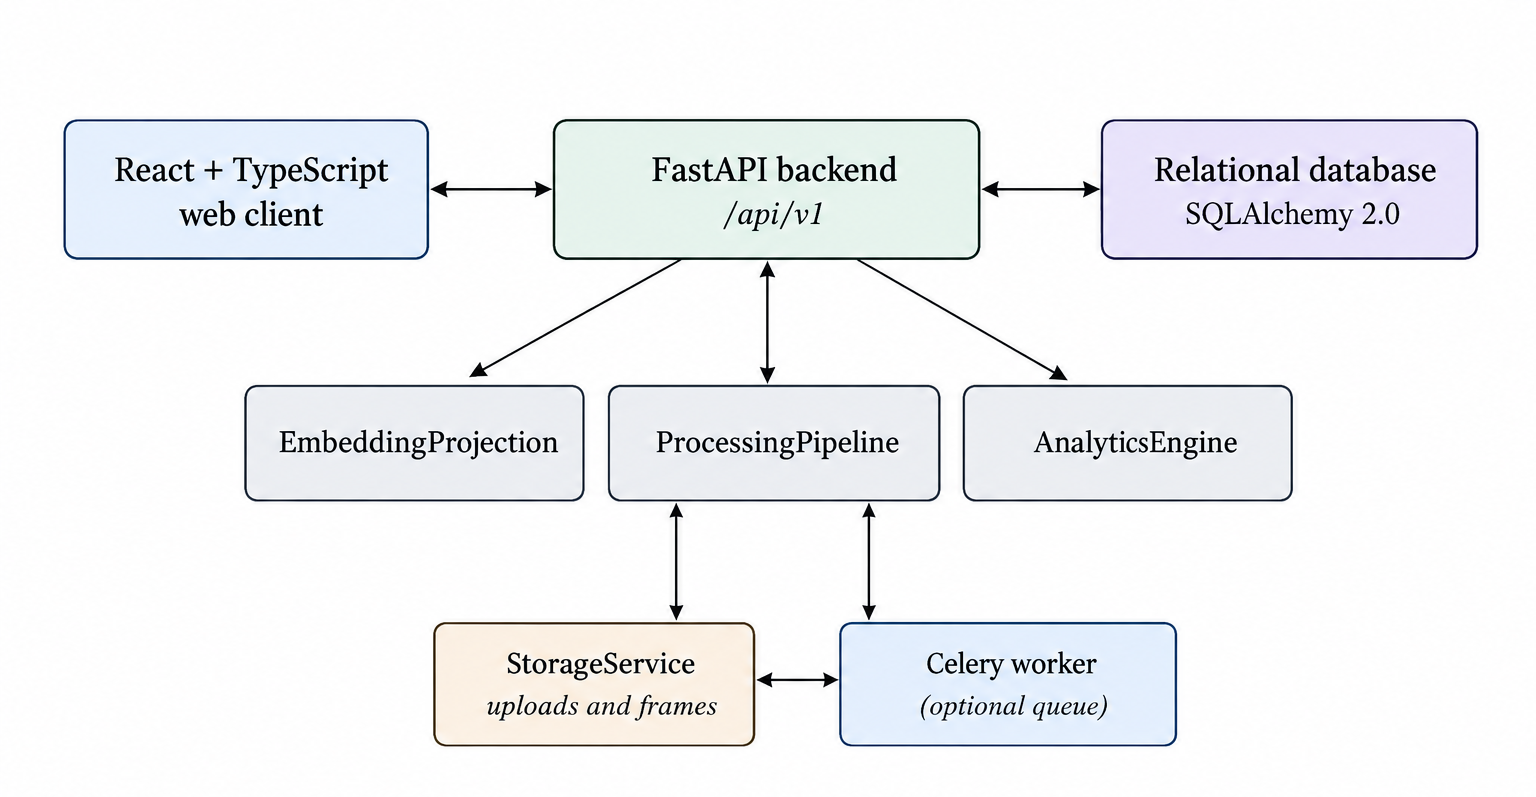
\includegraphics[width=0.95\linewidth]{architecture.png}
\caption[High-level architecture of OrchardVision]{High-level architecture of OrchardVision showing the web client, FastAPI backend, core services, relational database, file storage and optional Celery worker.}
\label{fig:arch}
\end{figure}

\section{Backend}

The backend is implemented with the following choices:

\begin{itemize}
  \item \textbf{Framework:} FastAPI with the SQLAlchemy~2.0 ORM.
  \item \textbf{Database:} SQLite, selected through the \code{DATABASE_URL} environment variable; the ORM layer allows a server database to be substituted without code changes.
  \item \textbf{API:} REST under \code{/api/v1/}, organised in router prefixes for health (\code{GET /health}), videos (\code{POST/GET/DELETE /videos}), tracks (\code{GET /videos/{id}/tracks}), identities (\code{GET /videos/{id}/identities}), processing (\code{POST /videos/{id}/process}), jobs (\code{GET /jobs/{id}}), experiments (\code{GET/POST/DELETE /experiments}) and settings (\code{GET/PUT /settings}).
\end{itemize}

\section{Frontend}

The frontend is a React and TypeScript application. Types shared with the API are defined once in \code{packages/types/src/}, the components live in \code{apps/web/src/}, and an API client calls the FastAPI backend. During development the Vite server proxies requests under \code{/api/} to the backend.

\section{Core Services}

\begin{itemize}
  \item \textbf{ProcessingPipeline.} Orchestrates frame extraction $\rightarrow$ detection $\rightarrow$ tracking $\rightarrow$ embedding $\rightarrow$ analytics.
  \item \textbf{EmbeddingProjection.} Produces t-SNE / PCA visualisations of identity prototypes, served as two-dimensional coordinates.
  \item \textbf{AnalyticsEngine.} Computes IDF1, HOTA and ID-switch metrics.
  \item \textbf{StorageService.} Saves uploads under \code{UPLOAD_DIR} and renders cached JPEG frames under \code{UPLOAD_DIR/frames/<video\_id>}, validating that resolved paths stay inside the upload directory.
\end{itemize}

\section{Configuration}

Configuration is loaded through \code{pydantic_settings} from an \code{.env} file. The key settings are the confidence threshold, the ReID threshold, the tracker type, the camera-motion mode, the memory update rate, the tracker match threshold and the number of buffer frames. The defaults are persisted in the \code{AppSettings} table, which holds a single row identified by \code{GLOBAL_SETTINGS_ID}, and can be read and updated through \code{GET /settings} and \code{PUT /settings}.

\section{Actors and Use Cases}

\add{Two kinds of users interact with the system. An \emph{analyst} (for example an agronomist or a student researcher) uploads videos, starts processing, inspects tracks and identities and reads analytics. An \emph{experimenter} additionally creates and compares experiments and edits the pipeline defaults. The main use cases are: upload video, process video, view tracks, view identities and their projection, view ReID events, view analytics, manage experiments, export results, edit settings and delete video.}

\figph{fig:usecase}{Use-case diagram}{Use-case diagram of OrchardVision.}{UML use-case diagram. Two actors on the left (Analyst, Experimenter) and the system boundary ``OrchardVision'' containing the ten use cases listed above. Draw Experimenter as a specialisation of Analyst, and connect ``Process video'' with an \texttt{include} relationship to ``Upload video''.}{6cm}

\section{Hardware and Software Requirements}

\begin{table}[htbp]
\centering\small
\begin{tabular}{@{}>{\raggedright\arraybackslash}p{3.6cm}>{\raggedright\arraybackslash}p{10.2cm}@{}}
\toprule
\hr \textbf{Item} & \textbf{Requirement}\\
\midrule
\hr Operating system & Linux, macOS or Windows capable of running Python, Node.js and Docker\\
\hr Python & Python environment with FastAPI, SQLAlchemy 2.0, pydantic-settings, uvicorn, Celery, OpenCV and the detection/tracking libraries used by the pipeline\\
\hr Node.js & Node.js with npm and pnpm for the frontend and the shared types package\\
\hr Database & SQLite\\
\hr File storage & Local disk through the storage service\\
\hr Compute & \pp{CPU / GPU model and memory used for the experiments}\\
\hr Browser & A current desktop browser (the frontend is served by Vite in development)\\
\bottomrule
\end{tabular}
\caption[Hardware and software requirements]{\add{Hardware and software requirements.}}
\label{tab:reqs}
\end{table}

\section{Technology Stack}

\begin{table}[htbp]
\centering\small
\begin{tabular}{@{}p{4.2cm}p{9.6cm}@{}}
\toprule
\textbf{Layer} & \textbf{Technology}\\
\midrule
Web framework & FastAPI served by uvicorn (gunicorn/uvicorn in production)\\
ORM / database & SQLAlchemy 2.0; SQLite (substitutable through \code{DATABASE_URL})\\
Settings & \code{pydantic_settings} loading \code{.env}\\
Background work & FastAPI background task, or Celery when a queue is configured\\
File storage & Local disk (uploads and frame cache)\\
Frontend & React, TypeScript, Vite\\
Shared contracts & TypeScript package in \code{packages/types/src/}\\
Testing / checks & \code{pytest}; \code{pnpm exec tsc --noEmit}\\
\bottomrule
\end{tabular}
\caption{Technology stack of OrchardVision.}
\label{tab:stack}
\end{table}

\section{Repository Organisation}

New models and migrations are added as SQLAlchemy~2.0 model definitions. New API routes live in \code{apps/api/app/routers/}, schemas in \code{apps/api/app/schemas/} and services in \code{apps/api/app/services/}. The application entry point and the global exception handler are in \code{apps/api/app/main.py}. The complete layout is given in Appendix~A.

\chapter{Data Model and Persistence}

\section{Introduction}

All results produced by the pipeline are persisted so that they can be retrieved later through the API without reprocessing the video. The data layer is defined with SQLAlchemy~2.0 model definitions. Most tables carry a \code{video_id} that links them to the \code{Video} row they were derived from, which is why deleting a video (\code{DELETE /videos/{id}}) removes all associated data.

\section{Entities}

Table~\ref{tab:models} lists the persisted models and their key fields.

{\singlespacing\small
\begin{longtable}{@{}p{3.8cm}p{10.2cm}@{}}
\caption{Data models and key fields.}\label{tab:models}\\
\toprule
\textbf{Model} & \textbf{Key fields}\\
\midrule
\endfirsthead
\toprule
\textbf{Model} & \textbf{Key fields}\\
\midrule
\endhead
\bottomrule
\endfoot
\code{Video} & \code{id}, \code{filename}, \code{width}, \code{height}, \code{fps}, \code{frame_count}, \code{status}\\
\code{ProcessingJob} & \code{id}, \code{video_id}, \code{status}, \code{stage}, \code{progress}, \code{config} (dict)\\
\code{Experiment} & \code{id}, \code{name}, \code{tracker}, \code{scenario}, \code{num_frames}, \code{status}, \code{metrics}\\
\code{IdentityRecord} & \code{id}, \code{video_id}, \code{identity_id}, \code{prototype} (embedding vector), \code{quality}, \code{observation_count}, \code{is_confident}\\
\code{Track} & \code{id}, \code{video_id}, \code{track_id}, \code{frames}, \code{first_seen}, \code{last_seen}\\
\code{DetectionRecord} & \code{id}, \code{video_id}, \code{frame_id}, \code{bbox}, \code{confidence}\\
\code{FrameTimingRecord} & \code{id}, \code{video_id}, \code{frame_id}, \code{proc_ms}\\
\code{CameraMotionRecord} & \code{id}, \code{video_id}, \code{motion_type}, \code{compensation_applied}\\
\code{IdentityObservation} & \code{id}, \code{video_id}, \code{identity_id}, \code{track_id}, \code{frame_id}\\
\code{ReidEvent} & \code{id}, \code{video_id}, \code{lost_frame_id}, \code{reappearance_frame_id}\\
\code{AppSettings} & \code{id} (=\code{GLOBAL_SETTINGS_ID}), \code{values} (dict)\\
\end{longtable}}

\section{Entity Relationships}

Figure~\ref{fig:er} gives an overview of how the models relate to each other. \add{The relationships shown are inferred from the \code{video_id}, \code{identity_id}, \code{track_id} and \code{frame_id} fields listed above; \code{Experiment} and \code{AppSettings} are independent of any single video.}

\begin{figure}[htbp]
\centering
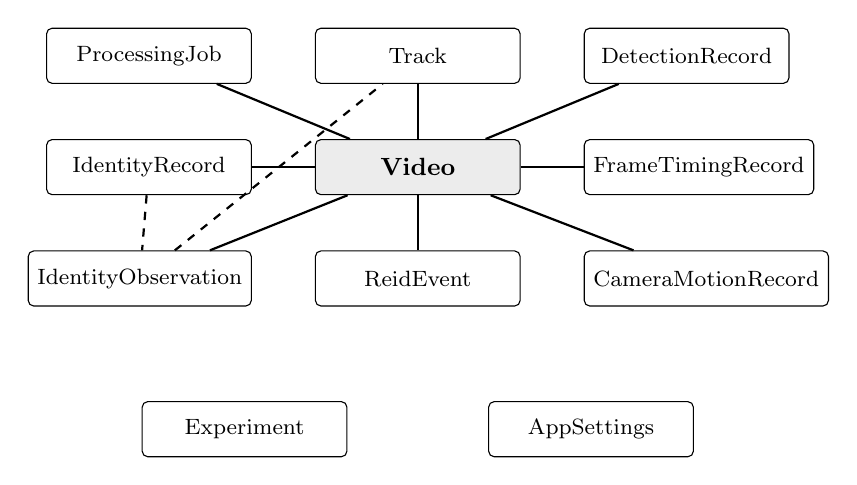
\begin{tikzpicture}[
  node distance=7mm and 8mm,
  ent/.style={draw,rounded corners=2pt,align=center,font=\footnotesize,minimum height=7mm,minimum width=2.6cm},
  main/.style={ent,fill=gray!15,font=\small\bfseries},
  lnk/.style={thick}]
\node[main] (video) {Video};
\node[ent,above left=of video] (job) {ProcessingJob};
\node[ent,above=of video] (track) {Track};
\node[ent,above right=of video] (det) {DetectionRecord};
\node[ent,left=of video] (ident) {IdentityRecord};
\node[ent,right=of video] (time) {FrameTimingRecord};
\node[ent,below left=of video] (obs) {IdentityObservation};
\node[ent,below=of video] (reid) {ReidEvent};
\node[ent,below right=of video] (cam) {CameraMotionRecord};
\node[ent,below=12mm of reid,xshift=-22mm] (exp) {Experiment};
\node[ent,below=12mm of reid,xshift=22mm] (set) {AppSettings};
\foreach \n in {job,track,det,ident,time,obs,reid,cam} \draw[lnk] (video) -- (\n);
\draw[lnk,dashed] (ident) -- (obs);
\draw[lnk,dashed] (obs) -- (track);
\end{tikzpicture}
\caption[Overview of the data model]{Overview of the data model: all per-video artefacts reference \code{Video}; \code{Experiment} and \code{AppSettings} are standalone.}
\label{fig:er}
\end{figure}

\section{Rows Created by One Processing Run}

When a processing job completes, the \code{Video} status becomes \code{processed} and the following rows are created: \code{IdentityRecord}, \code{Track}, \code{DetectionRecord}, \code{FrameTimingRecord} and \code{CameraMotionRecord}; identity sightings and re-identification events are stored as \code{IdentityObservation} and \code{ReidEvent} rows. Table~\ref{tab:rows} gives the template used to report the volume of data produced for a video.

\begin{table}[htbp]
\centering\small
\begin{tabular}{@{}lcc@{}}
\toprule
\hr \textbf{Model} & \textbf{Rows per video} & \textbf{Growth driver}\\
\midrule
\hr \code{DetectionRecord} & \pp{XX} & Frames $\times$ detections per frame\\
\hr \code{FrameTimingRecord} & \pp{XX} & One per processed frame\\
\hr \code{Track} & \pp{XX} & Number of tracks started\\
\hr \code{IdentityRecord} & \pp{XX} & Number of distinct fruit\\
\hr \code{IdentityObservation} & \pp{XX} & Sightings of identities\\
\hr \code{ReidEvent} & \pp{XX} & Occlusion/re-appearance events\\
\hr \code{CameraMotionRecord} & \pp{XX} & Motion estimate(s) for the video\\
\bottomrule
\end{tabular}
\caption[Rows per processed video]{\add{Rows created per processed video (counts to be filled in from a real run; the growth drivers are inferred).}}
\label{tab:rows}
\end{table}

\section{Identity Records}

An \code{IdentityRecord} stores the learned prototype of one fruit: an embedding vector, a quality score, the number of observations that contributed to it, and an \code{is_confident} flag. Each individual sighting of an identity in a frame, attributed to a track, is stored as an \code{IdentityObservation}. A \code{ReidEvent} records the frame in which an identity was lost and the frame in which it reappeared.

\add{This split keeps the compact summary (the prototype) separate from the evidence that produced it (the observations), which allows the interface to show both the identity-space visualisation and the per-frame history of any identity.}

\section{Tracks and Detections}

A \code{Track} holds the frames over which a tracker followed an object, together with its first and last frame. \code{DetectionRecord} stores the bounding box and confidence of each persisted detection. In the shared TypeScript types the bounding box is a \code{BoundingBox} with \code{x}, \code{y}, \code{width} and \code{height}, and a track point can be in one of three visibility states: \code{visible}, \code{occluded} or \code{lost}.

\section{Telemetry and Camera Motion}

\code{FrameTimingRecord} stores the processing time per frame in milliseconds (\code{proc_ms}) and is returned by \code{GET /videos/{id}/per-frame}. \code{CameraMotionRecord} stores the type of motion estimated for the video and whether compensation was applied, and is returned by \code{GET /videos/{id}/motion}.

\section{Settings and Experiments}

\code{AppSettings} is a single-row table whose \code{values} dictionary holds the pipeline defaults. \code{Experiment} stores the name, tracker, scenario, number of frames, status and computed metrics of an evaluation run. An experiment that is in the \code{RUNNING} state cannot be deleted.

\section{Database Selection}

SQLite is used throughout, with the development database file at \code{data/orchardvision.db} and the container stack pointing \code{DATABASE_URL} at a file in a shared volume. \add{Because all access goes through the SQLAlchemy ORM, the application code is identical whichever server is selected; only the connection string changes. The current limits of SQLite become visible with several concurrent writers, which is the main reason a deployment at scale would move to a server database. Every identifier is a 32-character hexadecimal UUID, and only the video-to-job relation is mapped as an ORM relationship; the remaining foreign keys are plain indexed columns, which keeps the persistence of high-volume tables such as detections and frame timings cheap.}

\chapter{Processing Pipeline and Identity Learning}

\section{Introduction}

This chapter explains how an uploaded video becomes a set of tracks, identities and analytics. It first describes the end-to-end flow (upload, process, retrieve), then each processing stage, the state models that describe progress, and the configuration parameters that control behaviour.

\section{End-to-End Flow}

\subsection{Upload}

The user posts a video to \code{POST /videos}. The backend saves the file through \code{storage_service.save_upload}, extracts its metadata with \code{extract_video_metadata}, and creates a \code{Video} row with status \code{uploaded}.

\subsection{Process}

A request to \code{POST /videos/{id}/process} first validates that there is no active job for the video. It then creates a \code{ProcessingJob} with status \code{QUEUED}, and either enqueues the work (Celery) or runs it synchronously as a background task. The background task performs:

\begin{enumerate}
  \item frame extraction according to the \code{PipelineConfig};
  \item object detection, using the model specified by \code{model_path};
  \item tracking, using the \code{mock}, \code{bytetrack} or \code{tapnext} tracker;
  \item re-identification embeddings;
  \item identity consolidation;
  \item analytics computation (\code{compute_video_analytics}).
\end{enumerate}

When processing finishes, the \code{Video} status becomes \code{processed}, and the \code{IdentityRecord}, \code{Track}, \code{DetectionRecord}, \code{FrameTimingRecord} and \code{CameraMotionRecord} rows are created.

\subsection{Retrieve}

The GET endpoints return the persisted tracks, identities, analytics, frame timings, motion estimates, ReID events and detections. Retrieval never triggers recomputation.

\begin{figure}[htbp]
\centering
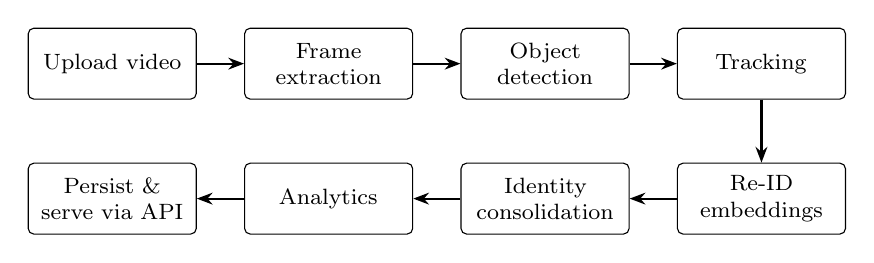
\begin{tikzpicture}[
  node distance=6mm,
  st/.style={draw,rounded corners=2pt,align=center,font=\footnotesize,minimum height=9mm,text width=1.9cm},
  arr/.style={-{Stealth[length=2mm]},thick}]
\node[st] (a) {Upload video};
\node[st,right=of a] (b) {Frame extraction};
\node[st,right=of b] (c) {Object detection};
\node[st,right=of c] (d) {Tracking};
\node[st,below=8mm of d] (e) {Re-ID embeddings};
\node[st,left=of e] (f) {Identity consolidation};
\node[st,left=of f] (g) {Analytics};
\node[st,left=of g] (h) {Persist \& serve via API};
\draw[arr] (a) -- (b);\draw[arr] (b) -- (c);\draw[arr] (c) -- (d);
\draw[arr] (d) -- (e);\draw[arr] (e) -- (f);\draw[arr] (f) -- (g);\draw[arr] (g) -- (h);
\end{tikzpicture}
\caption{Processing pipeline from upload to persisted results.}
\label{fig:pipeline}
\end{figure}

\section{Status Models}

The progress of a video and of a processing job is described by the shared TypeScript types in \code{packages/types/src/common.ts}:

\begin{itemize}
  \item \code{JobStatus}: \code{uploaded} $\rightarrow$ \code{processing} $\rightarrow$ \code{processed}, or \code{error};
  \item \code{ProcessingStage}: \code{frame_extraction} $\rightarrow$ \code{detection} $\rightarrow$ \code{tracking} $\rightarrow$ \code{reid} $\rightarrow$ \code{analytics};
  \item \code{ProcessingStatus}: \code{QUEUED} $\rightarrow$ \code{RUNNING} $\rightarrow$ \code{COMPLETED}, or \code{FAILED}.
\end{itemize}

\begin{figure}[htbp]
\centering
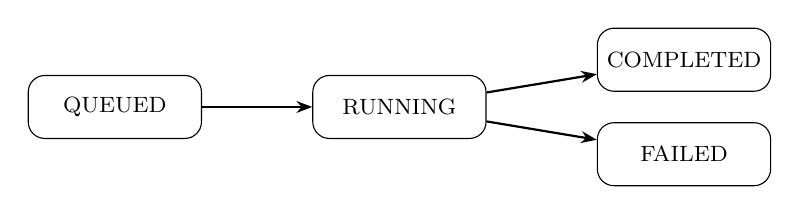
\begin{tikzpicture}[
  node distance=14mm,
  s/.style={draw,rounded corners=6pt,align=center,font=\footnotesize,minimum height=8mm,minimum width=2.2cm},
  arr/.style={-{Stealth[length=2mm]},thick}]
\node[s] (q) {QUEUED};
\node[s,right=of q] (r) {RUNNING};
\node[s,right=of r,yshift=6mm] (c) {COMPLETED};
\node[s,right=of r,yshift=-6mm] (f) {FAILED};
\draw[arr] (q) -- (r);\draw[arr] (r) -- (c);\draw[arr] (r) -- (f);
\end{tikzpicture}
\caption{Life cycle of a \texttt{ProcessingJob} (\texttt{ProcessingStatus}).}
\label{fig:jobstate}
\end{figure}

\section{Processing Stages}

\subsection{Frame Extraction}

Frames are extracted from the uploaded video according to the \code{PipelineConfig} of the job. The extracted frames are stored through the \code{StorageService} in MinIO/S3, where the video's width, height, frame rate and frame count were recorded at upload time. \add{Sub-sampling the frame rate reduces cost on long videos but increases the displacement of fruit between sampled frames, so it directly affects tracker difficulty.}

\subsection{Object Detection}

Fruit are detected in each frame by the model specified by \code{model_path}. Detections below the configured confidence threshold are discarded, and the remainder are persisted as \code{DetectionRecord} rows with their bounding box and confidence.

\subsection{Tracking}

The tracker links detections across frames into tracks. The tracker type is selected from \code{mock}, \code{bytetrack} and \code{tapnext}; the tracker match threshold and the number of buffer frames (how long an unmatched track is kept alive) are configurable. \add{The \code{mock} tracker provides a deterministic back-end for development and tests, ByteTrack is a motion-based tracking-by-detection baseline, and TAPNext follows points through the video (see Chapter~2).}

\subsection{Re-Identification Embeddings}

For each tracked detection the pipeline computes a ReID embedding. The embeddings are used to compare observations with the prototypes of existing identities, using the ReID threshold to decide whether a match is acceptable.

\subsection{Identity Consolidation}

Identity consolidation turns tracks and embeddings into persistent identities. For each identity the pipeline stores a prototype embedding, a quality score, the observation count and an \code{is_confident} flag; every sighting is recorded as an \code{IdentityObservation}. When an identity is lost and later reappears, a \code{ReidEvent} stores the lost frame and the reappearance frame.

\add{A common formulation for maintaining the prototype $\mathbf{p}_k$ of identity $k$ is an exponential moving average of the embeddings assigned to it, controlled by the memory update rate $\alpha$:}

\begin{equation}
\colorbox{\phcol}{$\displaystyle \mathbf{p}_k \leftarrow \frac{(1-\alpha)\,\mathbf{p}_k + \alpha\,\mathbf{e}_t}{\left\lVert (1-\alpha)\,\mathbf{p}_k + \alpha\,\mathbf{e}_t\right\rVert_2}$}
\end{equation}

\add{A detection with embedding $\mathbf{e}_t$ is re-associated with identity $k$ when the cosine similarity between $\mathbf{e}_t$ and $\mathbf{p}_k$ exceeds the ReID threshold $\tau_{\mathrm{reid}}$. This equation illustrates the role of the memory update rate; the exact update rule should be confirmed against the implementation before submission.}

\subsection{Analytics}

The analytics stage runs \code{compute_video_analytics}, which uses the \code{AnalyticsEngine} to compute IDF1, HOTA and the number of ID switches. The aggregated analytics are served by \code{GET /videos/{id}/analytics}.

\section{Stage Inputs and Outputs}

\begin{table}[htbp]
\centering\small
\begin{tabular}{@{}>{\raggedright\arraybackslash}p{2.9cm}>{\raggedright\arraybackslash}p{3.7cm}>{\raggedright\arraybackslash}p{3.7cm}>{\raggedright\arraybackslash}p{3.1cm}@{}}
\toprule
\textbf{Stage} & \textbf{Input} & \textbf{Output} & \textbf{Persisted as}\\
\midrule
Frame extraction & Uploaded video, \code{PipelineConfig} & Frames & Frames in object storage\\
Detection & Frames, \code{model_path}, confidence threshold & Bounding boxes with confidence & \code{DetectionRecord}\\
Tracking & Detections, tracker type, match threshold, buffer frames & Tracks & \code{Track}\\
ReID & Tracked detections & Embeddings & (used by next stage)\\
Identity consolidation & Tracks, embeddings, ReID threshold, memory update rate & Identity prototypes, observations, ReID events & \code{IdentityRecord}, \code{IdentityObservation}, \code{ReidEvent}\\
Analytics & Tracks, identities & IDF1, HOTA, ID switches, timings, motion & \code{FrameTimingRecord}, \code{CameraMotionRecord}\\
\bottomrule
\end{tabular}
\caption[Stage inputs and outputs]{Inputs, outputs and persisted records of each pipeline stage. \add{The input and output columns are summarised from the pipeline description; they are not an exhaustive interface specification.}}
\label{tab:stages}
\end{table}

\section{Camera Motion}

The camera motion of each video is estimated and stored in a \code{CameraMotionRecord} with its motion type and whether compensation was applied. The camera-motion mode is one of the pipeline settings. \add{Compensating for ego-motion before association keeps motion predictions meaningful when the camera moves along an orchard row.}

\section{Identity-Space Visualisation}

The \code{EmbeddingProjection} service reduces identity prototypes to two dimensions with t-SNE or PCA, so that the interface can display them. The coordinates are served by \code{GET /videos/{id}/identities/projection}. \add{Identities of the same fruit should form tight clusters, and well-separated clusters suggest that the ReID threshold is set sensibly.}

\section{Identity Consolidation Procedure}

\add{The listing below gives a simplified, illustrative description of how tracks and embeddings can be consolidated into identities. It is provided to explain the idea and does not reproduce the source code of the implementation.}

\begin{lstlisting}[style=added,language=Python,mathescape=false]
for track in tracks_sorted_by_first_seen:
    e = mean_embedding(track)
    k, sim = nearest_identity(e, identities)   # cosine similarity
    if k is not None and sim >= reid_threshold:
        assign(track, identities[k])
        record_reid_event_if_gap(track, identities[k])
        update_prototype(identities[k], e, alpha)
    else:
        identities.append(new_identity(track, e))
for k in identities:
    k.quality = mean_quality(k.observations)
    k.is_confident = k.observation_count >= min_obs
\end{lstlisting}

\add{In this scheme a track that begins after another has ended is compared with all existing prototypes; if the similarity exceeds the ReID threshold it inherits the identity and a ReID event (lost frame, reappearance frame) is stored. Otherwise a new identity is created. Tracks that overlap in time must not be merged into the same identity, which acts as a simple constraint against merging two different fruit.}

\section{Design Considerations}

\begin{itemize}
  \item \add{\textbf{Threshold trade-off.} A low ReID threshold merges different fruit (undercounting); a high one fragments one fruit into several identities (overcounting). The threshold is therefore exposed as a setting and evaluated through experiments.}
  \item \add{\textbf{Prototype memory.} A small memory update rate makes prototypes stable but slow to adapt to lighting changes; a large one adapts quickly but can drift towards a neighbouring fruit.}
  \item \add{\textbf{Separation of stages.} Persisting detections, tracks, embeddings-derived identities and timings separately makes it possible to diagnose in which stage a counting error originated.}
  \item \add{\textbf{Tracker as a plug-in.} Because the mock, ByteTrack and TAPNext trackers are selected by a setting, a new tracker can be compared with the existing ones using the same video, detector and metrics.}
\end{itemize}

\section{Computational Considerations}

\add{Detection and embedding extraction dominate the processing time per frame; association and identity matching grow with the number of active tracks and identities. The per-frame timing records stored for each video allow these costs to be measured on the actual hardware, which is the basis of the runtime study in Chapter~8.}

\section{Pipeline Parameters}

\begin{table}[htbp]
\centering\small
\begin{tabular}{@{}>{\raggedright\arraybackslash}p{4.3cm}>{\raggedright\arraybackslash}p{9.5cm}@{}}
\toprule
\textbf{Parameter} & \textbf{Purpose}\\
\midrule
Confidence threshold & \add{Minimum detector confidence for a detection to be kept}\\
ReID threshold & \add{Minimum similarity for re-associating an observation with an existing identity}\\
Tracker type & Selects the tracker: \code{mock}, \code{bytetrack} or \code{tapnext}\\
Camera motion mode & \add{Selects how camera motion is estimated and compensated}\\
Memory update rate & \add{Controls how quickly an identity prototype adapts to new observations}\\
Tracker match threshold & \add{Minimum score for linking a detection to an existing track}\\
Buffer frames & \add{Number of frames an unmatched track is retained before it is considered lost}\\
\bottomrule
\end{tabular}
\caption{Key pipeline parameters (defaults stored in \texttt{AppSettings}).}
\label{tab:params}
\end{table}

\section{Failure Handling}

\add{A processing job can end in the \code{FAILED} state, and the corresponding video in the \code{error} state, for example when the video cannot be decoded or a stage raises an exception. Because every stage persists its output, the cause of a failure can be located from the \code{stage} recorded on the job. A failed video can be deleted with \code{DELETE /videos/{id}} and uploaded again after the problem is fixed.}

\section{Reproducibility}

\add{Each \code{ProcessingJob} stores the configuration it ran with in its \code{config} dictionary, and each experiment stores its tracker, scenario and number of frames together with the resulting metrics. Together with the exports in JSON or CSV, this makes it possible to repeat an evaluation and to attach the exact configuration to every number reported in Chapter~8.}

\section{Concurrency and Job Control}

A video can have only one active processing job: requesting processing while a job is active is rejected (\add{the API defines a \code{ConflictError} for this kind of situation}). The state of a job (\code{status}, \code{stage}, \code{progress}) can be polled through \code{GET /jobs/{id}}. When the work is enqueued through Celery it runs outside the API process; otherwise it runs as a background task of the API process.

\chapter{API Design and Implementation}

\section{Introduction}

All functionality of OrchardVision is exposed through a REST API under the \code{/api/v1/} prefix. The same API is used by the React client and can be called directly by scripts. This chapter lists the endpoints, explains the request flows, and describes error handling and the shared TypeScript types.

\section{Endpoint Summary}

Table~\ref{tab:api} summarises the endpoints.

{\singlespacing\small
\begin{longtable}{@{}p{1.5cm}p{6.6cm}p{5.8cm}@{}}
\caption{REST API endpoints.}\label{tab:api}\\
\toprule
\textbf{Method} & \textbf{Path} & \textbf{Description}\\
\midrule
\endfirsthead
\toprule
\textbf{Method} & \textbf{Path} & \textbf{Description}\\
\midrule
\endhead
\bottomrule
\endfoot
GET & \code{/health} & Service health\\
POST & \code{/videos} & Upload video\\
GET & \code{/videos} & List videos\\
GET & \code{/videos/{id}} & Video metadata\\
GET & \code{/videos/{id}/tracks} & Track trajectories\\
GET & \code{/videos/{id}/identities} & Identity prototypes\\
GET & \code{/videos/{id}/identities/projection} & 2D coordinates for visualisation\\
GET & \code{/videos/{id}/identities/{identity_id}} & Specific identity\\
GET & \code{/videos/{id}/identities/{identity_id}/observations} & Per-frame observations\\
GET & \code{/videos/{id}/reid-events} & Re-identification events\\
GET & \code{/videos/{id}/detections} & Persisted detections\\
GET & \code{/videos/{id}/per-frame} & Per-frame timing telemetry\\
GET & \code{/videos/{id}/motion} & Camera motion estimate\\
GET & \code{/videos/{id}/analytics} & Aggregated analytics\\
DELETE & \code{/videos/{id}} & Delete video and all associated data\\
POST & \code{/videos/{id}/process} & Start processing job\\
GET & \code{/jobs/{id}} & Job status\\
GET & \code{/experiments} & List experiments\\
POST & \code{/experiments} & Create and run experiment\\
GET & \code{/experiments/{id}} & Experiment detail\\
GET & \code{/experiments/{id}/export} & Download results (JSON/CSV)\\
DELETE & \code{/experiments/{id}} & Delete experiment (cannot be \code{RUNNING})\\
GET & \code{/settings} & Pipeline defaults\\
PUT & \code{/settings} & Update pipeline defaults\\
\end{longtable}}

\section{Resource-to-Model Mapping}

Each read endpoint returns data that the pipeline persisted in one of the models of Chapter~4 (Table~\ref{tab:map}).

\begin{table}[htbp]
\centering\small
\begin{tabular}{@{}>{\raggedright\arraybackslash}p{5.9cm}>{\raggedright\arraybackslash}p{3.7cm}>{\raggedright\arraybackslash}p{3.8cm}@{}}
\toprule
\textbf{Endpoint} & \textbf{Model} & \textbf{Created in stage}\\
\midrule
\code{/videos/{id}} & \code{Video} & Upload\\
\code{/videos/{id}/tracks} & \code{Track} & Tracking\\
\code{/videos/{id}/detections} & \code{DetectionRecord} & Detection\\
\code{/videos/{id}/identities} & \code{IdentityRecord} & Identity consolidation\\
\code{/videos/{id}/identities/{identity_id}/observations} & \code{IdentityObservation} & Identity consolidation\\
\code{/videos/{id}/reid-events} & \code{ReidEvent} & Re-identification\\
\code{/videos/{id}/per-frame} & \code{FrameTimingRecord} & All stages\\
\code{/videos/{id}/motion} & \code{CameraMotionRecord} & Camera-motion estimation\\
\code{/videos/{id}/analytics} & Aggregated metrics & Analytics\\
\code{/jobs/{id}} & \code{ProcessingJob} & Process request\\
\code{/experiments} & \code{Experiment} & Experiment request\\
\code{/settings} & \code{AppSettings} & Settings update\\
\bottomrule
\end{tabular}
\caption[Endpoint-to-model mapping]{Mapping between endpoints and the persisted models. \add{The ``stage'' column is inferred from the pipeline description.}}
\label{tab:map}
\end{table}

\figph{fig:seq}{Sequence diagram of a processing request}{Sequence of calls for uploading and processing a video.}{UML sequence diagram with lifelines: Client, FastAPI router, StorageService, Database, Celery/background task, ProcessingPipeline. Messages: POST /videos $\rightarrow$ save\_upload $\rightarrow$ extract\_video\_metadata $\rightarrow$ insert Video (uploaded); POST /videos/\{id\}/process $\rightarrow$ validate no active job $\rightarrow$ insert ProcessingJob (QUEUED) $\rightarrow$ enqueue; worker updates stage and progress; final persistence and Video status processed; client polls GET /jobs/\{id\}.}{7cm}

\section{Request Flows}

\subsection{Video Upload}

\code{POST /videos} saves the upload through \code{storage_service.save_upload}, extracts metadata with \code{extract_video_metadata} and creates the \code{Video} row with status \code{uploaded}. The maximum upload size is 2\,GB by default and can be changed through \code{MAX_UPLOAD_BYTES}.

\subsection{Starting a Processing Job}

\code{POST /videos/{id}/process} validates that no job is active for the video, creates a \code{ProcessingJob} with status \code{QUEUED}, and then enqueues it with Celery or runs it synchronously as a background task. The client polls \code{GET /jobs/{id}} to read the job's \code{status}, \code{stage} and \code{progress}.

\subsection{Reading Results}

After a video is \code{processed}, its tracks, identities, observations, ReID events, detections, per-frame timing, camera motion and analytics are retrieved with the GET endpoints in Table~\ref{tab:api}. The identity projection endpoint returns two-dimensional coordinates computed by the \code{EmbeddingProjection} service for plotting.

\subsection{Experiments}

\code{POST /experiments} creates and runs an experiment described by a name, a tracker, a scenario and a number of frames. Its results can be read with \code{GET /experiments/{id}} and downloaded as JSON or CSV with \code{GET /experiments/{id}/export}. An experiment that is \code{RUNNING} cannot be deleted.

\subsection{Settings}

\code{GET /settings} and \code{PUT /settings} read and update the pipeline defaults stored in the single \code{AppSettings} row.

\section{Error Handling}

All errors are returned in a single format:

\begin{lstlisting}[style=plain]
{"detail": "...", "code": "...", "status": ...}
\end{lstlisting}

The API defines a base \code{ApiError} and the custom exceptions \code{NotFoundError}, \code{ConflictError} and \code{ValidationFailError}. A global exception handler in \code{apps/api/app/main.py} converts them into the response format above.

\section{Shared TypeScript Types}

Common interfaces are defined in \code{packages/types/src/common.ts} and are used by the frontend and by any other TypeScript client:

\begin{itemize}
  \item \code{BoundingBox}: \code{{ x: number, y: number, width: number, height: number }};
  \item \code{VisibilityState}: \code{'visible' | 'occluded' | 'lost'};
  \item \code{JobStatus}: \code{'uploaded' | 'processing' | 'processed' | 'error'};
  \item \code{ProcessingStage}: \code{'frame_extraction'}, \code{'detection'}, \code{'tracking'}, \code{'reid'}, \code{'analytics'};
  \item \code{ProcessingStatus}: \code{'QUEUED'}, \code{'RUNNING'}, \code{'COMPLETED'}, \code{'FAILED'};
  \item response wrappers such as \code{MultiVideoResponse}, \code{MultiTrackResponse} and \code{MultiIdentityResponse}.
\end{itemize}

The types can be checked with \code{pnpm exec tsc --noEmit} from \code{packages/types/}.

\section{Frontend Integration}

The components in \code{apps/web/src/} use an API client that calls the FastAPI backend. During development the Vite dev server (\code{npm run dev}) proxies requests under \code{/api/} to the backend, and the backend's CORS configuration allows \code{localhost:5173}. \add{The interface is organised around the main user tasks: uploading and listing videos, starting and monitoring processing, inspecting tracks and identities, viewing the identity projection, managing experiments and editing the pipeline settings.}

\section{Example Interaction}

\add{The following listing shows a typical sequence of calls for processing a video. The identifiers and the request body are illustrative.}

\begin{lstlisting}[style=added,language=bash]
# 1. upload a video
curl -F "file=@row_03.mp4" http://localhost:8000/api/v1/videos
# 2. start processing video 1 (tracker chosen in the body)
curl -X POST http://localhost:8000/api/v1/videos/1/process \
     -H "Content-Type: application/json" \
     -d '{"tracker": "bytetrack"}'
# 3. poll the job
curl http://localhost:8000/api/v1/jobs/1
# 4. read results
curl http://localhost:8000/api/v1/videos/1/analytics
\end{lstlisting}

\chapter{Deployment, Testing and Extension}

\section{Introduction}

This chapter describes how OrchardVision is run in development and production, how it is tested, and how developers extend it.

\section{Development Environment}

\begin{itemize}
  \item \textbf{Backend:} \code{uvicorn apps.api.app.main:app --reload}, with SQLite stored at \code{./data/app.db}.
  \item \textbf{Frontend:} \code{npm run dev} starts the Vite dev server, which proxies \code{/api/} to the backend.
  \item \textbf{CORS:} \code{localhost:5173} is configured as an allowed origin.
\end{itemize}

\section{Production Deployment}

In production the database is PostgreSQL, selected through \code{DATABASE_URL}. The API is served by gunicorn with uvicorn workers behind a reverse proxy. Uploads are limited to 2\,GB by default, configurable with the \code{MAX_UPLOAD_BYTES} environment variable. Videos and frames are stored through the \code{StorageService} in MinIO/S3.

\begin{figure}[htbp]
\centering
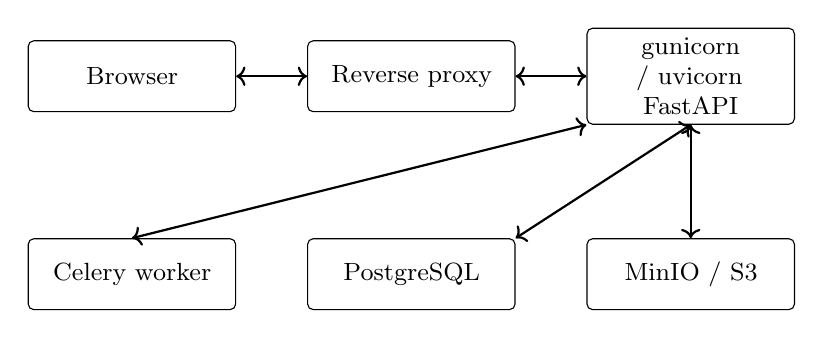
\begin{tikzpicture}[
  node distance=8mm and 9mm,
  b/.style={draw,rounded corners=2pt,align=center,font=\small,minimum height=9mm,text width=2.4cm},
  arr/.style={-{Stealth[length=2mm]},thick}]
\node[b] (c) {Browser};
\node[b,right=of c] (p) {Reverse proxy};
\node[b,right=of p] (g) {gunicorn / uvicorn\\FastAPI};
\node[b,below=16mm of p] (pg) {PostgreSQL};
\node[b,left=of pg] (w) {Celery worker};
\node[b,right=of pg] (s3) {MinIO / S3};
\draw[arr,<->] (c) -- (p);\draw[arr,<->] (p) -- (g);
\draw[arr,<->] (g.south) -- (pg.north east);
\draw[arr,<->] (g.south) -- (s3.north);
\draw[arr,<->] (g.south west) -- (w.north);
\end{tikzpicture}
\caption{Production deployment topology.}
\label{fig:deploy}
\end{figure}

\section{Configuration}

Settings are loaded with \code{pydantic_settings} from the \code{.env} file. The environment variables referred to in this report are \code{DATABASE_URL} (database selection) and \code{MAX_UPLOAD_BYTES} (upload limit). The pipeline defaults themselves are stored in the database and edited through the settings endpoints.

\section{Extending the System}

\begin{itemize}
  \item add new models and migrations as SQLAlchemy~2.0 model definitions;
  \item add new API routes in \code{apps/api/app/routers/};
  \item add new schemas in \code{apps/api/app/schemas/};
  \item add new services in \code{apps/api/app/services/}.
\end{itemize}

\section{Testing}

The Python test suite is run with \code{pytest} from the repository root, and the shared TypeScript types are type-checked with \code{pnpm exec tsc --noEmit} from \code{packages/types/}.

\add{The tests are organised around the layers of the system. The following cases are recommended to be covered and, where not yet automated, are listed here as a test plan:}

\begin{table}[htbp]
\centering\small
\begin{tabular}{@{}>{\raggedright\arraybackslash}p{1.2cm}>{\raggedright\arraybackslash}p{5.7cm}>{\raggedright\arraybackslash}p{6.7cm}@{}}
\toprule
\hr \textbf{ID} & \textbf{Test case} & \textbf{Expected result}\\
\midrule
\hr T1 & Upload a valid video & \code{Video} row created with status \code{uploaded} and correct metadata\\
\hr T2 & Start processing twice on the same video & Second request rejected while the first job is active\\
\hr T3 & Run a job with the \code{mock} tracker & Job moves \code{QUEUED}, \code{RUNNING}, \code{COMPLETED}; video becomes \code{processed}\\
\hr T4 & Request a non-existent video & Error JSON with \code{detail}, \code{code} and \code{status}\\
\hr T5 & Delete a video & Associated tracks, identities and detections are removed\\
\hr T6 & Delete a \code{RUNNING} experiment & Request rejected\\
\hr T7 & Export an experiment as CSV and JSON & Downloaded file contains the stored metrics\\
\hr T8 & Update settings and read them back & Updated values returned by \code{GET /settings}\\
\bottomrule
\end{tabular}
\caption[Recommended test plan]{\add{Recommended test plan.}}
\label{tab:tests}
\end{table}

\section{Security and Robustness Considerations}

\add{Because the system accepts large file uploads, deployments should enforce the upload limit at the reverse proxy as well as in the application, restrict the allowed CORS origins to the production front-end, and keep the object-store credentials in the environment rather than in the repository. Deleting a video removes all associated data, so the delete endpoint should be protected by authentication in multi-user deployments.}

\section{User Guide}

\add{This section describes the typical workflow of a user of the web interface. Screenshots of the relevant screens are in Chapter~8.}

\begin{enumerate}
  \item \add{\textbf{Start the services.} Start the backend with uvicorn and the frontend with Vite as shown in Section~7.2, and open the web client in a browser.}
  \item \add{\textbf{Review the settings.} Open the settings page and check the confidence threshold, ReID threshold, tracker type, camera-motion mode, memory update rate, tracker match threshold and buffer frames. Save the changes with the update action.}
  \item \add{\textbf{Upload a video.} Choose a video file (up to 2\,GB by default). When the upload completes, the video appears in the list with status \code{uploaded} together with its resolution, frame rate and frame count.}
  \item \add{\textbf{Start processing.} Select the video and start a processing job. The job moves from \code{QUEUED} to \code{RUNNING}; the current stage (frame extraction, detection, tracking, ReID, analytics) and progress are shown until the status becomes \code{COMPLETED}.}
  \item \add{\textbf{Inspect the results.} Open the tracks to see trajectories and visibility states, the identities to see prototypes, quality and observation counts, the identity projection to see how identities cluster, the ReID events to see where identities were lost and found again, and the analytics to read IDF1, HOTA and ID switches.}
  \item \add{\textbf{Run an experiment.} Create an experiment by choosing a tracker, a scenario and a number of frames, and wait for its status to change from \code{RUNNING}. Compare the metrics of several experiments and download them as JSON or CSV.}
  \item \add{\textbf{Clean up.} Delete videos and experiments that are no longer needed. Deleting a video removes all of its tracks, identities and other records.}
\end{enumerate}

\figph{fig:flow}{User workflow}{Flowchart of the user workflow.}{Flowchart with the seven steps above as boxes connected by arrows: Start services $\rightarrow$ Review settings $\rightarrow$ Upload video $\rightarrow$ Start processing $\rightarrow$ Inspect results $\rightarrow$ Run experiment $\rightarrow$ Clean up. Add a feedback arrow from Inspect results back to Review settings (``adjust thresholds'').}{4.5cm}

\section{Project Plan}

\add{Table~\ref{tab:plan} lists the phases of the project. The durations and dates are to be completed by the candidate.}

\begin{table}[htbp]
\centering\small
\begin{tabular}{@{}>{\raggedright\arraybackslash}p{1.1cm}>{\raggedright\arraybackslash}p{7.2cm}>{\raggedright\arraybackslash}p{2.6cm}>{\raggedright\arraybackslash}p{2.6cm}@{}}
\toprule
\hr \textbf{Phase} & \textbf{Activity} & \textbf{Start} & \textbf{End}\\
\midrule
\hr 1 & Literature survey and problem definition & \pp{date} & \pp{date}\\
\hr 2 & Data model and API design & \pp{date} & \pp{date}\\
\hr 3 & Processing pipeline and trackers & \pp{date} & \pp{date}\\
\hr 4 & Identity learning and analytics & \pp{date} & \pp{date}\\
\hr 5 & Web interface and experiment harness & \pp{date} & \pp{date}\\
\hr 6 & Testing, evaluation and report writing & \pp{date} & \pp{date}\\
\bottomrule
\end{tabular}
\caption[Project plan]{\add{Project plan (to be completed).}}
\label{tab:plan}
\end{table}

\section{Risk Analysis}

\begin{table}[htbp]
\centering\small
\begin{tabular}{@{}>{\raggedright\arraybackslash}p{4.3cm}>{\raggedright\arraybackslash}p{4.4cm}>{\raggedright\arraybackslash}p{4.9cm}@{}}
\toprule
\hr \textbf{Risk} & \textbf{Effect} & \textbf{Mitigation}\\
\midrule
\hr Very large uploads & Slow requests, disk pressure & 2\,GB limit (\code{MAX_UPLOAD_BYTES}); object storage\\
\hr Long-running processing & Blocked API workers & Background task or Celery queue; job polling\\
\hr Identity merges or fragmentation & Wrong fruit counts & Tunable ReID threshold; experiment harness\\
\hr Camera motion & Tracking drift & Camera-motion estimation and compensation\\
\hr Database growth & Slower queries & PostgreSQL in production; per-video deletion\\
\bottomrule
\end{tabular}
\caption[Risk analysis]{\add{Risks and mitigations.}}
\label{tab:risk}
\end{table}

\chapter{Experimental Evaluation and Results}

\section{Introduction}

\add{This chapter describes how OrchardVision is evaluated and provides the tables and figures into which the measured results are to be entered. No quantitative results are stated here: every value marked \texttt{\pp{XX.X}} and every image placeholder must be replaced with output from the project's own experiment runs before submission.}

\section{Experiment Harness}

The evaluation is performed with the experiment harness of the system. An experiment is created with \code{POST /experiments} and is described by a name, a tracker, a scenario and a number of frames. The harness runs the experiment, stores its status and metrics in the \code{Experiment} record, and allows the results to be downloaded as JSON or CSV with \code{GET /experiments/{id}/export}. The metrics computed by the \code{AnalyticsEngine} are IDF1, HOTA and the number of ID switches.

\section{Experimental Set-up}

\subsection{Data}

\add{Table~\ref{tab:dataset} is to be completed with the orchard videos used in the evaluation.}

\begin{table}[htbp]
\centering\small
\begin{tabular}{@{}lllllll@{}}
\toprule
\hr \textbf{Video} & \textbf{Orchard} & \textbf{Camera} & \textbf{Resolution} & \textbf{FPS} & \textbf{Frames} & \textbf{GT fruit}\\
\midrule
\hr V1 & \pp{...} & \pp{...} & \pp{...} & \pp{...} & \pp{...} & \pp{...}\\
\hr V2 & \pp{...} & \pp{...} & \pp{...} & \pp{...} & \pp{...} & \pp{...}\\
\hr V3 & \pp{...} & \pp{...} & \pp{...} & \pp{...} & \pp{...} & \pp{...}\\
\bottomrule
\end{tabular}
\caption[Evaluation videos]{\add{Videos used for evaluation (to be filled in).}}
\label{tab:dataset}
\end{table}

\begin{figure}[htbp]
\centering
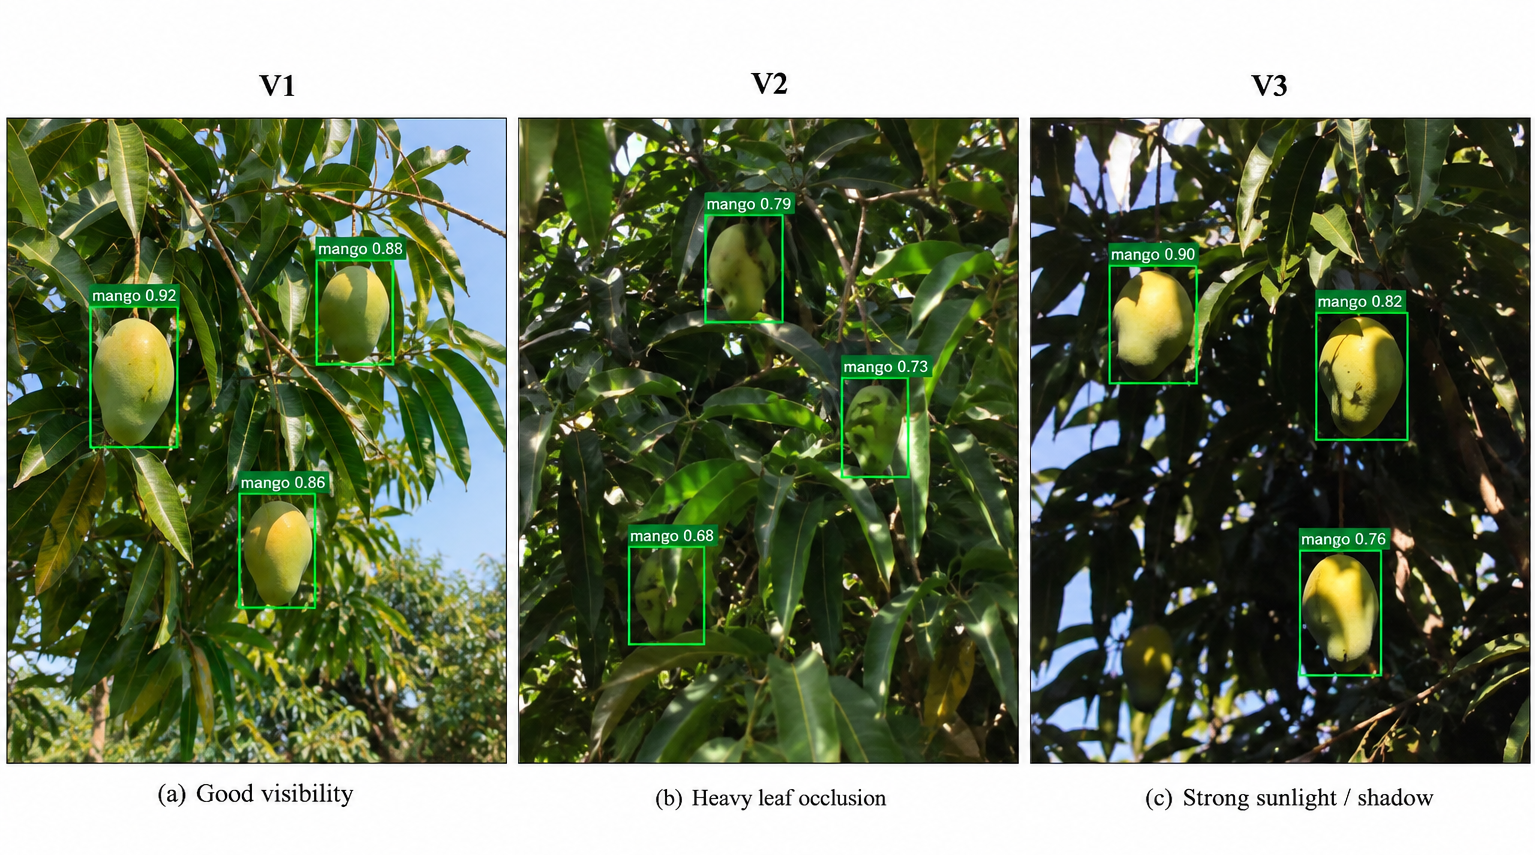
\includegraphics[width=0.95\linewidth]{frames.png}
\caption[Sample orchard frames]{Sample frames from the evaluation videos showing fruit under different illumination and occlusion.}
\label{fig:frames}
\end{figure}

\subsection{Configurations}

\add{The trackers listed in the system (mock, ByteTrack, TAPNext) are compared under identical detector, frame range and ReID settings. The camera-motion mode is varied to study the effect of compensation.}

\subsection{Metrics}

\add{IDF1, HOTA and the number of identity switches are reported for each configuration, as computed by the \code{AnalyticsEngine}. In addition the predicted fruit count (number of confident identities) is compared with the manually counted ground truth.}

\section{Tracker Comparison}

\begin{table}[htbp]
\centering\small
\begin{tabular}{@{}lcccc@{}}
\toprule
\hr \textbf{Tracker} & \textbf{IDF1 (\%)} & \textbf{HOTA (\%)} & \textbf{ID switches} & \textbf{Count error (\%)}\\
\midrule
\hr mock & \pp{XX.X} & \pp{XX.X} & \pp{XX} & \pp{XX.X}\\
\hr ByteTrack & \pp{XX.X} & \pp{XX.X} & \pp{XX} & \pp{XX.X}\\
\hr TAPNext & \pp{XX.X} & \pp{XX.X} & \pp{XX} & \pp{XX.X}\\
\bottomrule
\end{tabular}
\caption[Tracker comparison]{\add{Comparison of tracker back-ends on the evaluation videos (to be filled in from experiment exports).}}
\label{tab:trackers}
\end{table}

\figph{fig:bars}{Tracker comparison chart}{Bar chart comparing IDF1, HOTA and ID switches for the evaluated trackers.}{Grouped bar chart. X-axis: tracker (mock, ByteTrack, TAPNext). Two bars per tracker for IDF1 and HOTA on the left y-axis (0--100\%), and a line or secondary axis for the number of ID switches. Generate from the CSV exported by \texttt{GET /experiments/{id}/export}.}{5.2cm}

\section{Effect of Camera Motion Compensation}

\begin{table}[htbp]
\centering\small
\begin{tabular}{@{}lccc@{}}
\toprule
\hr \textbf{Camera-motion mode} & \textbf{IDF1 (\%)} & \textbf{HOTA (\%)} & \textbf{ID switches}\\
\midrule
\hr Off & \pp{XX.X} & \pp{XX.X} & \pp{XX}\\
\hr On (compensation applied) & \pp{XX.X} & \pp{XX.X} & \pp{XX}\\
\bottomrule
\end{tabular}
\caption[Camera motion ablation]{\add{Effect of camera-motion compensation (to be filled in).}}
\label{tab:cam}
\end{table}

\section{Identity Prototypes and Re-Identification}

\figph{fig:proj}{Identity embedding projection}{Two-dimensional projection of identity prototypes for one processed video.}{Scatter plot produced by the identity projection view (\texttt{GET /videos/{id}/identities/projection}) using t-SNE or PCA. Each point is an identity prototype; colour can encode the \texttt{is\_confident} flag and marker size the observation count. Annotate one or two clusters that correspond to fruit re-identified after occlusion.}{5.5cm}

\figph{fig:reid}{Re-identification example}{Example of an identity lost and re-identified after an occlusion.}{Filmstrip of four crops of the same fruit: (1) last frame before it is lost (\texttt{lost\_frame\_id}), (2) a frame in which it is hidden by leaves, (3) the reappearance frame (\texttt{reappearance\_frame\_id}), and (4) a later frame. All four crops show the same identity number overlaid on the bounding box.}{4.2cm}

\section{Sensitivity to the ReID Threshold}

\add{Table~\ref{tab:thr} is to be filled by running the same video with several ReID thresholds and recording the resulting identity count, IDF1 and identity switches.}

\begin{table}[htbp]
\centering\small
\begin{tabular}{@{}cccc@{}}
\toprule
\hr \textbf{ReID threshold} & \textbf{Identities found} & \textbf{IDF1 (\%)} & \textbf{ID switches}\\
\midrule
\hr \pp{0.5} & \pp{XX} & \pp{XX.X} & \pp{XX}\\
\hr \pp{0.6} & \pp{XX} & \pp{XX.X} & \pp{XX}\\
\hr \pp{0.7} & \pp{XX} & \pp{XX.X} & \pp{XX}\\
\hr \pp{0.8} & \pp{XX} & \pp{XX.X} & \pp{XX}\\
\bottomrule
\end{tabular}
\caption[ReID threshold sensitivity]{\add{Sensitivity of the results to the ReID threshold (to be filled in; threshold values are examples).}}
\label{tab:thr}
\end{table}

\figph{fig:thr}{Threshold sweep}{Identity count and IDF1 as a function of the ReID threshold.}{Line plot with the ReID threshold on the x-axis. Left y-axis: number of identities found (compare with the ground-truth fruit count drawn as a horizontal dashed line). Right y-axis: IDF1 (\%). The best operating point should be marked.}{5cm}

\section{Counting Accuracy}

\begin{table}[htbp]
\centering\small
\begin{tabular}{@{}lcccc@{}}
\toprule
\hr \textbf{Video} & \textbf{Ground truth} & \textbf{Predicted} & \textbf{Abs. error} & \textbf{Error (\%)}\\
\midrule
\hr V1 & \pp{XX} & \pp{XX} & \pp{XX} & \pp{XX.X}\\
\hr V2 & \pp{XX} & \pp{XX} & \pp{XX} & \pp{XX.X}\\
\hr V3 & \pp{XX} & \pp{XX} & \pp{XX} & \pp{XX.X}\\
\bottomrule
\end{tabular}
\caption[Counting accuracy]{\add{Fruit-count accuracy for the best configuration (to be filled in).}}
\label{tab:count}
\end{table}

\section{Runtime Performance}

\add{Per-frame processing times are stored as \code{FrameTimingRecord} rows and returned by \code{GET /videos/{id}/per-frame}. Table~\ref{tab:timing} summarises them per tracker.}

\begin{table}[htbp]
\centering\small
\begin{tabular}{@{}lccc@{}}
\toprule
\hr \textbf{Tracker} & \textbf{Mean (ms/frame)} & \textbf{95th percentile (ms)} & \textbf{Throughput (FPS)}\\
\midrule
\hr mock & \pp{XX} & \pp{XX} & \pp{XX}\\
\hr ByteTrack & \pp{XX} & \pp{XX} & \pp{XX}\\
\hr TAPNext & \pp{XX} & \pp{XX} & \pp{XX}\\
\bottomrule
\end{tabular}
\caption[Processing time]{\add{Processing time per frame (to be filled in; state the hardware used).}}
\label{tab:timing}
\end{table}

\figph{fig:timing}{Per-frame processing time}{Per-frame processing time over the course of one video.}{Line plot. X-axis: frame index; y-axis: \texttt{proc\_ms}. One line per tracker. Mark any spikes (for example model warm-up or large numbers of detections).}{5cm}

\section{Web Interface}

\add{The following screenshots document the web interface and should be captured from the running application.}

\figph{fig:ui_videos}{Video list and upload screen}{Video list and upload screen.}{Screenshot of the page that lists uploaded videos with their status (\texttt{uploaded}, \texttt{processing}, \texttt{processed}, \texttt{error}) and the upload control.}{4.5cm}

\figph{fig:ui_tracks}{Track visualisation}{Track overlay on a processed video.}{Screenshot of a processed video with bounding boxes and track trails drawn over a frame. Visible, occluded and lost states should be distinguishable (for example by solid, dashed and faded outlines).}{5cm}

\figph{fig:ui_exp}{Experiment management screen}{Experiment list and metrics view.}{Screenshot of the experiments page showing the list of experiments, their tracker, scenario, number of frames, status and metrics, together with the export (JSON/CSV) buttons.}{4.5cm}

\figph{fig:ui_set}{Settings screen}{Pipeline settings screen.}{Screenshot of the settings page showing the confidence threshold, ReID threshold, tracker type, camera-motion mode, memory update rate, tracker match threshold and buffer frames.}{4.5cm}

\section{Discussion}

\add{The discussion should interpret the numbers in Tables~\ref{tab:trackers} and \ref{tab:cam}: which tracker keeps identities longest through occlusion, whether camera-motion compensation reduces identity switches, how the ReID threshold trades merged identities against fragmented ones, and how the runtime per frame compares with the video frame rate. It should also include a short analysis of failure cases, such as fruit hidden for longer than the buffer, clusters of touching fruit, and fruit entering and leaving at the image border, supported by the examples in Figures~\ref{fig:reid} and \ref{fig:ui_tracks}.}

\chapter{Conclusion and Future Work}

\section{Conclusion}

OrchardVision delivers a complete system for long-term fruit tracking and counting in mango orchards. A FastAPI backend with a SQLAlchemy~2.0 data layer runs a processing pipeline (frame extraction, detection, tracking, ReID embedding, identity consolidation and analytics), persists every intermediate and final artefact, and exposes them through a documented REST API. A React and TypeScript frontend with shared type definitions provides video management, inspection of tracks and identities, and an experiment harness that evaluates trackers with IDF1, HOTA and ID-switch metrics and exports the results as JSON or CSV.

The main take-away points are:

\begin{itemize}
  \item identities are first-class, persistent objects (prototype, quality, observation count, confidence), which allows a fruit that disappears and reappears to be recognised rather than counted twice;
  \item the tracker back-end (mock, ByteTrack, TAPNext), camera-motion mode and thresholds are configurable and can be compared reproducibly through the experiment harness;
  \item the same code runs on a laptop with SQLite and as a container stack in which a queue worker processes the long-running jobs, so nothing about the pipeline depends on the deployment.
\end{itemize}

\add{Measured against the objectives of Section~1.5, the pipeline, data model, API, experiment harness and deployment configuration are in place. The accuracy objectives can only be claimed once Chapter~8 has been populated with results from real orchard videos; until then the quality of the counts should be treated as unverified. A realistic limitation is that identity matching rests on appearance embeddings of visually similar fruit, so merged or fragmented identities are expected in dense clusters and after very long gaps.}

\section{Future Work}

\add{The following extensions would increase the value of the system:}

\begin{itemize}
  \item \add{evaluate on a larger, annotated, multi-season mango dataset and publish the results;}
  \item \add{fine-tune the ReID network on fruit crops with a metric-learning loss and compare prototype aggregation strategies;}
  \item \add{replace the monocular heuristics with depth or multi-camera information to resolve fruit that occlude each other;}
  \item \add{link identities across recording sessions to track individual fruit through the season (the long-term setting);}
  \item \add{estimate fruit size and maturity for yield-weight prediction;}
  \item \add{add authentication and role-based access control for multi-user deployments;}
  \item \add{add live-stream ingestion and incremental processing so that counts update while the video is being recorded.}
\end{itemize}

\chapter*{References}
\addcontentsline{toc}{chapter}{REFERENCES}
\begin{small}
\singlespacing
\setlength{\parskip}{5pt}
\begin{list}{}{\setlength{\leftmargin}{2.2em}\setlength{\itemindent}{-2.2em}\setlength{\labelwidth}{0pt}\setlength{\labelsep}{0pt}\setlength{\itemsep}{4pt}\setlength{\parsep}{0pt}}
\item[] \add{[1].\ Aharon, N., Orfaig, R., \& Bobrovsky, B.-Z. (2022). BoT-SORT: Robust associations multi-pedestrian tracking. \emphon{}arXiv preprint arXiv:2206.14651\emphoff{}.}
\item[] \add{[2].\ Bargoti, S., \& Underwood, J. (2017). Deep fruit detection in orchards. In \emphon{}Proceedings of the IEEE International Conference on Robotics and Automation (ICRA)\emphoff{} (pp.\ 3626--3633). IEEE.}
\item[] \add{[3].\ Bayer, M. (2012). SQLAlchemy. In A. Brown \& G. Wilson (Eds.), \emphon{}The Architecture of Open Source Applications, Volume II\emphoff{}. aosabook.org.}
\item[] \add{[4].\ Bernardin, K., \& Stiefelhagen, R. (2008). Evaluating multiple object tracking performance: The CLEAR MOT metrics. \emphon{}EURASIP Journal on Image and Video Processing, 2008\emphoff{}, Article 246309.}
\item[] \add{[5].\ Bewley, A., Ge, Z., Ott, L., Ramos, F., \& Upcroft, B. (2016). Simple online and realtime tracking. In \emphon{}Proceedings of the IEEE International Conference on Image Processing (ICIP)\emphoff{} (pp.\ 3464--3468). IEEE.}
\item[] \add{[6].\ Doersch, C., Gupta, A., Markeeva, L., Recasens, A., Smaira, L., Aytar, Y., Carreira, J., Zisserman, A., \& Yang, Y. (2022). TAP-Vid: A benchmark for tracking any point in a video. In \emphon{}Advances in Neural Information Processing Systems (NeurIPS), Datasets and Benchmarks Track\emphoff{}.}
\item[] \add{[7].\ Hermans, A., Beyer, L., \& Leibe, B. (2017). In defense of the triplet loss for person re-identification. \emphon{}arXiv preprint arXiv:1703.07737\emphoff{}.}
\item[] \add{[8].\ Kalman, R. E. (1960). A new approach to linear filtering and prediction problems. \emphon{}Journal of Basic Engineering, 82\emphoff{}(1), 35--45.}
\item[] \add{[9].\ Koirala, A., Walsh, K. B., Wang, Z., \& McCarthy, C. (2019). Deep learning -- Method overview and review of use for fruit detection and yield estimation. \emphon{}Computers and Electronics in Agriculture, 162\emphoff{}, 219--234.}
\item[] \add{[10].\ Kuhn, H. W. (1955). The Hungarian method for the assignment problem. \emphon{}Naval Research Logistics Quarterly, 2\emphoff{}(1--2), 83--97.}
\item[] \add{[11].\ Liu, X., Chen, S. W., Liu, C., Shivakumar, S. S., Das, J., Taylor, C. J., Underwood, J., \& Kumar, V. (2019). Monocular camera based fruit counting and mapping with semantic data association. \emphon{}IEEE Robotics and Automation Letters, 4\emphoff{}(3), 2296--2303.}
\item[] \add{[12].\ Luiten, J., Ošep, A., Dendorfer, P., Torr, P., Geiger, A., Leal-Taixé, L., \& Leibe, B. (2021). HOTA: A higher order metric for evaluating multi-object tracking. \emphon{}International Journal of Computer Vision, 129\emphoff{}(2), 548--578.}
\item[] \add{[13].\ Ramírez, S. (n.d.). \emphon{}FastAPI\emphoff{} [Computer software]. https://fastapi.tiangolo.com}
\item[] \add{[14].\ Redmon, J., Divvala, S., Girshick, R., \& Farhadi, A. (2016). You only look once: Unified, real-time object detection. In \emphon{}Proceedings of the IEEE Conference on Computer Vision and Pattern Recognition (CVPR)\emphoff{} (pp.\ 779--788). IEEE.}
\item[] \add{[15].\ Ristani, E., Solera, F., Zou, R., Cucchiara, R., \& Tomasi, C. (2016). Performance measures and a data set for multi-target, multi-camera tracking. In \emphon{}European Conference on Computer Vision Workshops\emphoff{} (pp.\ 17--35). Springer.}
\item[] \add{[16].\ Wojke, N., Bewley, A., \& Paulus, D. (2017). Simple online and realtime tracking with a deep association metric. In \emphon{}Proceedings of the IEEE International Conference on Image Processing (ICIP)\emphoff{} (pp.\ 3645--3649). IEEE.}
\item[] \add{[17].\ Zhang, Y., Sun, P., Jiang, Y., Yu, D., Weng, F., Yuan, Z., Luo, P., Liu, W., \& Wang, X. (2022). ByteTrack: Multi-object tracking by associating every detection box. In \emphon{}European Conference on Computer Vision (ECCV)\emphoff{} (pp.\ 1--21). Springer.}
\item[] \add{[18].\ Zholus, A., Doersch, C., Yang, Y., Koppula, S., Patraucean, V., He, X. O., Rocco, I., Sajjadi, M. S. M., Chandar, S., \& Goroshin, R. (2025). TAPNext: Tracking any point (TAP) as next token prediction. \emphon{}arXiv preprint arXiv:2504.05579\emphoff{}.}
\item[] \add{[19].\ Ester, M., Kriegel, H.-P., Sander, J., \& Xu, X. (1996). A density-based algorithm for discovering clusters in large spatial databases with noise. In \emphon{}Proceedings of the Second International Conference on Knowledge Discovery and Data Mining (KDD)\emphoff{} (pp.\ 226--231). ACM.}
\item[] \add{[20].\ Jolliffe, I. T., \& Cadima, J. (2016). Principal component analysis: A review and recent developments. \emphon{}Philosophical Transactions of the Royal Society A, 374\emphoff{}(2015.02052).}
\item[] \add{[21].\ van der Maaten, L., \& Hinton, G. (2008). Visualizing data using t-SNE. \emphon{}Journal of Machine Learning Research, 9\emphoff{}(Nov), 2579--2605.}
\item[] \add{[22].\ Reddi, R., Kreibich, G., Poffenbarger, N., \& Chandra, R. (2017). A loss function for deep metric learning. In \emphon{}Proceedings of the IEEE International Conference on Computer Vision (ICCV)\emphoff{} (pp.\ 4187--4195). IEEE.}
\item[] \add{[23].\ YOLO Team \& Ultralytics (2024). \emphon{}Ultralytics YOLO\emphoff{} [Computer software]. https://github.com/ultralytics/ultralytics}
\end{list}
\end{small}

\clearpage
\chapter*{Appendix 1: Repository Layout}
\addcontentsline{toc}{chapter}{APPENDIX 1: REPOSITORY LAYOUT}

The directories referred to in the project documentation are shown below.

\begin{lstlisting}[style=plain]
apps/
  api/
    app/
      main.py          # FastAPI app and global exception handler
      routers/         # API routes
      schemas/         # request / response schemas
      services/        # ProcessingPipeline, EmbeddingProjection,
                       # AnalyticsEngine, StorageService
  web/
    src/               # React components and API client
packages/
  types/
    src/
      common.ts        # shared TypeScript types
data/
  app.db               # SQLite database (development)
\end{lstlisting}

\chapter*{Appendix 2: Run Commands}
\addcontentsline{toc}{chapter}{APPENDIX 2: RUN COMMANDS}

\begin{lstlisting}[style=plain]
# backend (development, SQLite at ./data/app.db)
uvicorn apps.api.app.main:app --reload

# frontend (Vite dev server, proxies /api/ to the backend)
npm run dev

# tests
pytest

# type-check the shared types (from packages/types/)
pnpm exec tsc --noEmit
\end{lstlisting}

\chapter*{Appendix 3: Illustrative API Responses}
\addcontentsline{toc}{chapter}{APPENDIX 3: ILLUSTRATIVE API RESPONSES}

\add{The following responses are illustrative: the field names follow the data model in Chapter~4, while the values and the exact response envelope are examples and should be replaced with real output from the running system.}

\textbf{GET /api/v1/jobs/1}
\begin{lstlisting}[style=added]
{
  "id": 1,
  "video_id": 1,
  "status": "RUNNING",
  "stage": "tracking",
  "progress": 0.45,
  "config": {"tracker": "bytetrack"}
}
\end{lstlisting}

\textbf{GET /api/v1/videos/1/identities/7}
\begin{lstlisting}[style=added]
{
  "id": 7,
  "video_id": 1,
  "identity_id": 7,
  "prototype": [0.021, -0.113, "..."],
  "quality": 0.82,
  "observation_count": 143,
  "is_confident": true
}
\end{lstlisting}

\textbf{GET /api/v1/videos/1/reid-events}
\begin{lstlisting}[style=added]
[
  {"id": 3, "video_id": 1,
   "lost_frame_id": 412, "reappearance_frame_id": 466}
]
\end{lstlisting}

\textbf{Error response (404)}
\begin{lstlisting}[style=added]
{"detail": "Video 99 not found", "code": "not_found", "status": 404}
\end{lstlisting}


\end{document}
